%questions not yet added
\باب{ غیر معاصر ترتیبی ادوار }\شناخت{باب_غیر_معاصر}
وسیع پیمانہ عددی ادوار عموماً معاصر ادوار کے طرز پر بنائے جاتے ہیں۔ان کے اگلے حال مکمل طور پر موجودہ حال سے حاصل ہوتے ہیں۔ حال صرف ساعت کے کنارے پر تبدیل ہوتے ہیں اور باقی اوقات کے لئے انہیں غیر متغیر تصور کیا جا سکتا ہے۔ساعت کے کنارے سے چند لمحات قبل تا چند لمحات بعد تک تمام حال کا پائیدار ہونا یقینی بنایا جاتا ہے۔یوں کنارہ ساعت پر معلوم حال پائے جاتے ہیں جن سے اگلے پر یقین حال حاصل ہوتے ہیں۔ 

اس کے برعکس غیر معاصر ادوار کے حال کسی بھی لمحہ تبدیل ہو سکتے ہیں جس سے حالت دوڑ اور دیگر مسائل کھڑے ہوتے ہیں جن پر اس باب میں غور کیا جائے گا۔

غیر معاصر ادوار کی اپنی ایک اہمیت ہے۔یہ ساعت کے کنارے کا انتظار کیے بغیر اشارہ کو ردعمل کر سکتے ہیں۔عموماً کسی بھی عددی دور میں کچھ حصہ معاصر اور کچھ غیر معاصر ہو گا۔

شکل \حوالہ{شکل_غیر_معاصر_لرزش} میں نہایت سادہ دور دکھایا گیا ہے جس کو سرسری نظر سے دیکھ کر یوں محسوس ہوتا ہے کہ ضرب گیٹ کا مخارج کبھی بلند نہیں ہو سکتا۔غور کرنے سے ثابت ہوتا ہے کہ مسئلہ اتنا سادہ نہیں۔ جب بھی مداخل \عددی{A} حال تبدیل کرے اس کے چند لمحوں بعد نفی گیٹ کا مخارج حال تبدیل کرے گا۔یہ \اصطلاح{ تاخیر }\فرہنگ{تاخیر}\حاشیہب{delay}\فرہنگ{delay} نفی گیٹ کے \اصطلاح{دورانیہ ردِ عمل } کی بدولت ہے۔شکل میں \عددی{A} اور \عددی{\overline{A}} کے خط کھینچتے ہوئے یہ تاخیر بڑھا چڑھا کر  دکھائی گئی ہے۔اگر ضرب گیٹ کا دورانیہ ردِ عمل صفر ہوتا تب ضرب گیٹ کا مخارج ان دو مداخل کے مطابق حال \عددی{Y_0} اختیار کرتا۔حقیقتاً ضرب گیٹ کو بھی ردِ عمل کے لئے چند لمحات درکار ہوں گے لہٰذا ضرب گیٹ کا مخارج \عددی{Y} ہو گا۔

\begin{figure}
\centering
\begin{subfigure}{1\textwidth}
\centering
\begin{tikzpicture}
\pgfmathsetmacro{\klen}{1};
\pgfmathsetmacro{\kpin}{0.5};
\pgfmathsetmacro{\kpina}{0.75};
\pgfmathsetmacro{\ksepX}{1.1}
\pgfmathsetmacro{\ksepY}{2}
\pgfmathsetmacro{\ksepYa}{1.1}
\pgfmathsetmacro{\ksepdX}{0.2}
\draw(0,0)node[and port,scale=1,number inputs=2,scale=1,anchor=out](u0){}  (u0.out)node[right]{$Y$};
\draw(u0.in 2)--++(0,-\kpin)--++(-\kpin,0)node[above]{$\overline{A}$}node[not port,anchor=out,scale=0.8](u1){};
\draw(u0.in 1)--(u0.in 1 -| u1.in)--++(-2*\kpin,0)coordinate(aa)node[left]{$A$};
\draw(u1.in)--++(-\kpin,0)coordinate(bb)--(bb |- aa);
\end{tikzpicture}
\caption{}
\end{subfigure}
\begin{subfigure}{1\textwidth}
\centering
 \begin{tikzpicture}
  \pgfmathsetmacro{\kH}{0.75}
   \pgfmathsetmacro{\ksepY}{\kH+0.5}
\draw[thick](0,0)node[above left]{$A$}--++(2,0)--++(0,\kH)--++(5,0)--++(0,-\kH)--++(2,0);
\draw[thick](0,-\ksepY)node[above left]{$\overline{A}$}  (0,-\ksepY+\kH)--++(3,0)--++(0,-\kH)--++(5,0)--++(0,\kH)--++(1,0);
\draw[thick](0,-2*\ksepY)node[above left]{$Y_0$}--++(2,0)--++(0,\kH)--++(1,0)--++(0,-\kH)--++(6,0);
\draw[thick](0,-3*\ksepY)node[above left]{$Y$}--++(3.25,0)--++(0,\kH)--++(1,0)coordinate[pos=0.5](kglitch)--++(0,-\kH)--++(4.75,0);
\draw[dashed](2,\kH)++(0,0.2)--++(0,0.5)coordinate(aa)  (3,-\ksepY+\kH)++(0,0.2)coordinate(bbN)--(bbN |- aa) coordinate(bb);
\draw[stealth-stealth]($(aa)+(0,-0.2)$)--($(bb)+(0,-0.2)$)coordinate[pos=0.5](ka);
\draw(ka)++(0,0.2) to [out=90,in=0]++(-1,0.5)node[left]{\RL{نفی گیٹ کا دورانیہ رد عمل}};
\draw[dashed](2,-2*\ksepY)++(0,-0.2)--++(0,-\ksepY-0.7)coordinate(cc)  (3.25,-3*\ksepY)++(0,-0.2)coordinate(ddP)--(ddP |- cc)coordinate(dd);
\draw[stealth-stealth]($(cc)+(0,0.2)$)--($(dd)+(0,0.2)$)coordinate[pos=0.5](kb);
\draw(kb)++(0,-0.2) to [out=-90,in=180]++(1,-0.5)node[right]{\RL{ضرب گیٹ کا دورانیہ رد عمل}};
\draw(kglitch)++(0,0.2) to [out=90,in=180]++(0.5,0.75)node[right]{\RL{لرزش}};
\end{tikzpicture}
\caption{}
\end{subfigure}
\caption{مثبت برقی لرزش۔}
\label{شکل_غیر_معاصر_لرزش}
\end{figure}

آپ دیکھ سکتے ہیں ضرب گیٹ کا مخارج غیر مطلوبہ طور پر ، نفی گیٹ کے دورانیہ ردِ عمل کے برابر دورانیے کے لئے، بلند ہو گا۔اس طرح کے ، غیر مطلوبہ نہایت کم دورانیہ کے لئے ،حال کی تبدیلی کو\اصطلاح{ برقی لرزش} یا مختصراً \اصطلاح{ لرزش}\فرہنگ{لرزش}\حاشیہب{glitch}\فرہنگ{glitch} کہتے ہیں۔ برقی لرزش مثبت یا منفی ہو سکتی ہے لہٰذا موجودہ لرزش کو مثبت لرزش کہیں گے۔ لرزش نہایت کم دورانیے کی دھڑکن تصور کی جا سکتی ہے، تاہم لرزش کی اصطلاح عموماً غیر مطلوبہ دھڑکن کے لئے استعمال کی جاتی ہے اور ان سے معاصر ادوار کو پاک رکھا جاتا ہے۔

 لرزش کی وجہ سے ادوار \اصطلاح{عبوری حال }\فرہنگ{عبوری حال } \حاشیہب{transition state}\فرہنگ{state!transition} اختیار کرتے ہیں۔اس باب میں عبوری حال پر تفصیلاً بحث ہو گی۔ 

آپ نے دیکھا کہ ضرب گیٹ تک اشارہ \عددی{\overline{A}} پہنچنے میں تاخیر کی بدولت لرزش پیدا ہوئی۔تاخیر کی مزید ایک مثال دیکھتے ہیں۔

برقی تار میں برقی دباو کی رفتار تقریباً خلاء میں روشنی کی رفتار \حاشیہب{خلاء میں روشنی کی رفتار \عددی{3\times 10^8} میٹر فی سیکنڈ ہے۔}کے برابر ہوتی ہے۔یوں ایک نینو سیکنڈ میں برقی دباو تقریباً \عددی{3\times 10^8\times 10^{-9}=0.3} میٹر یعنی \عددی{30} سنٹی میٹر فاصلہ طے کرتا ہے۔آئیے دیکھتے ہیں اگر پچھلی مثال تبدیل کر کے نفی گیٹ کی جگہ \عددی{30} سینٹی میٹر برقی تار لگائی جائے اور ضرب گیٹ کی جگہ بلا شرکت جمع گیٹ نصب کیا جائے تو دور کا ردِ عمل کیسا ہوگا ( شکل \حوالہ{شکل_غیر_معاصر_لمبائی_تار_لرزش} دیکھیں)۔

\begin{figure}
\centering
\begin{subfigure}{1\textwidth}
\centering
\begin{tikzpicture}
\pgfmathsetmacro{\klen}{1};
\pgfmathsetmacro{\kpin}{0.5};
\pgfmathsetmacro{\kpina}{0.25};
\pgfmathsetmacro{\ksepX}{1.1}
\pgfmathsetmacro{\ksepY}{2}
\pgfmathsetmacro{\ksepYa}{1.1}
\pgfmathsetmacro{\ksepdX}{0.2}
\draw(0,0)node[xor port,number inputs=2,scale=1](u0){};
\path($(u0.in 1)!0.5!(u0.in 2)$)++(0,0.5*\kpina)coordinate(kup);
\draw(u0.out)node[right]{$Y$};
\draw(u0.in 1)--++(0,2*\kpin)coordinate[pos=0.75](kst)node[above]{$A$};
\draw(u0.in 1)--++(-\kpin,0)--++(0,\kpin)--++(-\kpina,0)--++(0,-\kpin)--++(-\kpina,0)--++(0,\kpin)--++(-\kpina,0)--++(0,-\kpin)--++(-\kpina,0)--++(0,\kpin)--++(-\kpina,0)--++(0,-\kpin)--++(-\kpina,0)--++(0,\kpin)--++(-\kpina,0)--++(0,-\kpin)--++(-\kpina,0)--++(0,\kpin)--++(-\kpina,0)--++(0,-\kpin)coordinate(aaa)--(aaa |- kup)--++(-\kpin,0)coordinate(kmid)--++(0,-\kpina)--++(\kpin,0)coordinate(cc)--(cc |- u0.in 2)--++(0,-\kpin)coordinate(kbot)--++(\kpina,0)--++(0,\kpin)--++(\kpina,0)--++(0,-\kpin)--++(\kpina,0)--++(0,\kpin)--++(\kpina,0)--++(0,-\kpin)--++(\kpina,0)--++(0,\kpin)--++(\kpina,0)--++(0,-\kpin)--++(\kpina,0)--++(0,\kpin)--++(\kpina,0)--++(0,-\kpin)--++(\kpina,0)coordinate(kend)--++(0,\kpin)--(u0.in 2)node[below,xshift=-1ex]{$A_t$};
\draw[stealth-stealth](kst)--(kst-| kmid)--++(-1.5*\kpin,0)coordinate(ktop)--(ktop |- kbot)coordinate[pos=0.5](ktxt)--++(0,-0.5*\kpin)coordinate(kklft)--(kklft -| u0.in 2);
\draw(ktxt)node[fill=white,xshift=-0.5cm]{\RL{تیس سنٹی میٹر}};
\end{tikzpicture}
\caption{}
\end{subfigure}
\begin{subfigure}{1\textwidth}
\centering
 \begin{tikzpicture}
  \pgfmathsetmacro{\kH}{0.75}
   \pgfmathsetmacro{\ksepY}{\kH+0.5}
\draw[thick](0,0)node[above left]{$A$}--++(2,0)--++(0,\kH)--++(5,0)--++(0,-\kH)--++(4,0);
\draw[thick](0,-\ksepY)node[above left]{$A_t$}--++(3,0)--++(0,\kH)--++(5,0)--++(0,-\kH)--++(3,0);
\draw[thick](0,-2*\ksepY)node[above left]{$Y_0$}--++(2,0)--++(0,\kH)--++(1,0)--++(0,-\kH)--++(4,0)--++(0,\kH)--++(1,0)--++(0,-\kH)--++(3,0);
\draw[thick](0,-3*\ksepY)node[above left]{$Y$}--++(3.25,0)--++(0,\kH)--++(1,0)coordinate[pos=0.5](kglitch)--++(0,-\kH)--++(4,0)--++(0,\kH)--++(1,0)coordinate[pos=0.5](kglitchA)--++(0,-\kH)--++(1.75,0);
\draw[dashed](2,\kH)++(0,0.2)--++(0,0.5)coordinate(aa)  (3,-\ksepY+\kH)++(0,0.2)coordinate(bbN)--(bbN |- aa) coordinate(bb);
\draw[stealth-stealth]($(aa)+(0,-0.2)$)--($(bb)+(0,-0.2)$)coordinate[pos=0.5](ka);
\draw(ka)++(0,0.2) to [out=90,in=0]++(-1,0.5)node[left]{\RL{ایک نینو سیکنڈ}};
\draw[dashed](2,-2*\ksepY)++(0,-0.2)--++(0,-\ksepY-0.7)coordinate(cc)  (3.25,-3*\ksepY)++(0,-0.2)coordinate(ddP)--(ddP |- cc)coordinate(dd);
\draw[stealth-stealth]($(cc)+(0,0.2)$)--($(dd)+(0,0.2)$)coordinate[pos=0.5](kb);
\draw(kb)++(0,-0.2) to [out=-90,in=180]++(1,-0.5)node[right]{\RL{بلا شرکت جمع  گیٹ کا دورانیہ رد عمل}};
\draw(kglitch)++(0,0.2) to [out=90,in=180]++(0.5,0.75)node[right]{\RL{لرزش}};
\draw(kglitchA)++(0,0.2) to [out=90,in=180]++(0.5,0.75)node[right]{\RL{لرزش}};
\end{tikzpicture}
\caption{}
\end{subfigure}
\caption{دو برقی تاروں کی لمبائی میں فرق کی بدولت پیدا لرزشیں۔}
\label{شکل_غیر_معاصر_لمبائی_تار_لرزش}
\end{figure}

 اشارہ \عددی{A} گیٹ کے ایک داخلی پن پر مہیا کیا گیا ہے جبکہ یہی اشارہ تیس سنٹی میٹر برقی تار سے گزار کر دوسرے داخلی پن پر مہیا کیا گیا ہے جہاں  (تاخیر سے پہنچنے والے) اشارے کو \عددی{A_t} کہا گیا ہے۔ تار کو بل دار لکیر سے ظاہر کیا گیا ہے۔یوں اشارہ \عددی{A_t} گیٹ کے دوسرے پن تک (تار میں ترسیل کے بعد) \موٹا{  تاخیر } سے پہنچتا ہے۔اشارہ \عددی{A} بلند یا پست ہونے کے ایک نینو سیکنڈ بعد اشارہ \عددی{A_t} بلند یا پست ہو گا۔گیٹ کا دورانیہ ردِ عمل نظر انداز کرتے ہوئے گیٹ کا مخارج \عددی{Y_0} ہوگا۔ گیٹ کا دورانیہ ردِ عمل مدِ نظر رکھتے ہوئے مخارج \عددی{Y} ہوگا۔گیٹ کے خارجی اشارے میں دو بلند برقی لرزشیں دیکھنے کو ملتی ہیں جن کے دورانیے برقی تار میں تاخیر کے برابر ہیں۔یوں اشارے کی راہ میں تاخیر، حافظہ کی طرح، معلومات لمحاتی طور یاد رکھنے کی صلاحیت رکھتی ہیں۔

آپ نے دیکھا مختلف طرز کی تاخیر دور میں لرزشیں پیدا کرتی ہیں۔جہاں\اصطلاح{ باز رسی اشارہ }\فرہنگ{باز رسی اشارہ}\حاشیہب{feedback signal}\فرہنگ{feedback signal} تاخیر سے پہنچ کر مخارج تبدیل کرتا ہو وہاں دوران تاخیر مخارج اور تاخیر کے بعد مخارج مختلف ہوں گے جس سے \اصطلاح{ نا پائیدار حالت }\فرہنگ{حالت!نا پائیدار}\حاشیہب{unstable condition}\فرہنگ{unstable condition} پیدا ہو گی۔

 جب بھی ایک سے زیادہ اشارے بیک وقت تبدیل ہوں، گیٹ اور برقی تاروں میں نا قابل معلوم تاخیر کی بدولت ، ان کے اثرات جاننا تقریباً ناممکن ہو گا۔اس مسئلے سے بچنے کی خاطر غیر معاصر ادوار درج ذیل دو شرائط کے تحت بنائے جاتے ہیں: (ا) ایک وقت پر صرف ایک اشارہ تبدیل ہو؛ (ب) اشاروں کی تبدیلی کے درمیان اتنا وقفہ دیا جائے کہ تاخیر کے باوجود دور پائیدار حال اختیار کرتا ہو۔ان شرائط کے تحت چلنے کو \اصطلاح{بنیادی طریق کار }\فرہنگ{بنیادی طریقہ کار}\حاشیہب{fundamental mode}\فرہنگ{fundamental mode} کے تحت چلنا کہتے ہیں۔

\حصہ{ تجزیہ}
\اصطلاح{غیر معاصر ترتیبی ادوار }\فرہنگ{ترتیبی دور!غیر معاصر}\حاشیہب{asynchronous combinational circuit}\فرہنگ{asynchronous!combinational circuit} سے مراد ایسے ادوار ہیں جن میں (ا) بغیر ساعت والے پلٹ پائے جائیں اور یا (ب) ان میں ایک یا ایک سے زیادہ مخارج بطور \اصطلاح{ باز رسی اشارات } استعمال ہوں۔جیسے اُوپر ذکر کیا گیا،مختلف نوعیت کی تاخیر کی بنا پر باز رسی اشارات لمحاتی طور پر حافظہ کی صلاحیت رکھتے ہیں۔

جب خارجی اشارہ، مثلاً \عددی{D}، بطور داخلی اشارہ استعمال ہو کر اپنی ہی قیمت \عددی{(D)} تعین کرنے میں کردار ادا کر تا ہو، یہ \اصطلاح{باز رسی اشارہ }\فرہنگ{باز رسی اشارہ}\حاشیہب{feedback signal}\فرہنگ{feedback signal} کہلاتا ہے۔

اس حصہ میں بغیر پلٹ ادوار پر غور کیا جائے گا۔پلٹ والے دور پر اگلے حصہ میں غور کیا جائے گا۔

\جزوحصہ{عبوری جدول}
غیر معاصر ترتیبی ادوار پر غور ان کے \اصطلاح{ عبوری جدول }\فرہنگ{عبوری جدول}\حاشیہب{transition table}\فرہنگ{transition table} کی مدد سے کیا جاتا ہے۔یہ طریقہ شکل   \حوالہ{شکل_غیر_معاصر_دور_کی_مثال}  میں دیے گئے دور کی مدد سے سیکھتے ہیں۔

\begin{figure}
\centering
\begin{tikzpicture}
\pgfmathsetmacro{\klen}{1};
\pgfmathsetmacro{\kpin}{0.5};
\pgfmathsetmacro{\kpina}{0.25};
\pgfmathsetmacro{\ksepX}{1.1}
\pgfmathsetmacro{\ksepY}{2}
\pgfmathsetmacro{\ksepYa}{1.1}
\pgfmathsetmacro{\ksepdX}{0.2}
\draw(0,0)node[and port,number inputs=2,scale=1,anchor=out](u0){};
\draw(0,\ksepY)node[and port,number inputs=2,scale=1,anchor=out](u1){};
\draw[thin](u1.in 1)--++(0,\kpin)--++(-\kpin,0)node[or port,scale=1,number inputs=2,anchor=out](u2){};
\draw[thin](u1.in 2)--++(-\kpin,0)--++(0,-\kpin)node[or port,scale=1,anchor=out,number inputs=2](u3){};
\draw[thin](u0.in 2)--++(-\kpin,0)node[or port,scale=1,number inputs=2,anchor=out](u4){};
\draw[thin](u1.in 1)--(u0.in 1);
\draw[thin](u4.in 2)--++(-\kpin,0)node[not port,anchor=out,scale=0.8](u5){};
\draw[thin](u3.in 1)--++(-\kpin,0)node[not port,anchor=out,scale=0.8](u6){};
\draw[thin](u6.out)|-(u4.in 1);
\draw[thin](u3.in 2)--++(0,-\kpin)-|(u5.in)node[left]{$a$} --++(0,-2*\kpin)-|(u1.out)--++(\kpin,0)node[right]{$A$};
\draw[thin](u0.out)--++(\kpin,0)coordinate[pos=0.5](kB)node[right]{$B$};
\draw[thin](u2.in 1)node[above left]{$b$}--++(0,2*\kpin)-|(kB);
\draw[thin](u2.in 2)--(u2.in 2-| u5.in)--++(-\kpin,0)node[left]{$X$};
\draw[thin](u6.in)--(u6.in |- u2.in 2);
\end{tikzpicture}
\caption{غیر معاصر دور۔}
\label{شکل_غیر_معاصر_دور_کی_مثال}
\end{figure}

پلٹ کی غیر موجودگی کے باوجود اس کو ترتیبی دور اس لئے کہیں گے کہ خارجی اشارے \عددی{A} اور \عددی{B} بطور  \اصطلاح{باز رسی اشارات}\فرہنگ{باز رسی اشارات}\حاشیہب{feedback signals}\فرہنگ{feedback signals} ، \عددی{a} اور \عددی{b}، استعمال کیے گئے ہیں۔دور سے خارجی حال کی مساوات لکھتے ہیں۔
\begin{gather}
\begin{aligned}
A&=(b+x)\cdot (a+\overline{x})\\
B&=(b+x)\cdot (\overline{a}+\overline{x})
\end{aligned}
\end{gather}
مساوات حاصل کرتے وقت باز رسی اشاروں کو عام مداخل تصور کریں۔یوں \عددی{x} کو بیرونی مداخل جبکہ \عددی{a} اور \عددی{b} کو اندرونی مداخل تصور کریں۔ ان مساوات میں \عددی{a} اور \عددی{b} \موٹا{ موجودہ مخارج } جبکہ \عددی{A} اور \عددی{B} \موٹا{ اگلے مخارج }ہیں۔ ان مساوات سے جدول \حوالہ{جدول_غیر_معاصر_باز رسی} حاصل ہو گا جس سے عبوری جدول کا حصول شکل  \حوالہ{شکل_غیر_معاصر_عبوری_جدول_حصول}  میں دکھایا گیا ہے۔
\begin{table}
\caption{دور کا بوولین جدول۔}
\label{جدول_غیر_معاصر_باز رسی}
\centering
\begin{otherlanguage}{english}
\begin{tabular}{CCC|CC}
\toprule
a&b&x&A&B\\
\midrule
0&0&0&0&0\\
0&0&1&0&1\\
0&1&0&1&1\\
0&1&1&0&1\\
1&0&0&1&1\\
1&0&1&1&0\\
1&1&0&0&0\\
1&1&1&1&0\\
\bottomrule
\end{tabular}
\end{otherlanguage}
\end{table}
%

\begin{figure}
\centering
\begin{tikzpicture}
\pgfmathsetmacro{\kxstep}{1}
\pgfmathsetmacro{\kystep}{1}
\pgfmathsetmacro{\kpin}{0.75}
\pgfmathsetmacro{\ksepX}{2*\kxstep+2}
\foreach \x in {0,1,2}{\draw(1*\ksepX+\x*\kxstep,0)--++(0,-4*\kystep);}
\foreach \x in {0,1,2,3,4}{\draw(1*\ksepX,-\x*\kystep)--++(2*\kxstep,0);}
\draw(\ksepX,0)--++(135:\kpin)node[pos=0.75,above right]{$x$}node[pos=0.75,below left]{$ab$};
\foreach \kx/\xlb in {0/{0},1/{1}}{\draw(\ksepX+\kx*\kxstep+\kxstep/2,0)node[above]{$\xlb$};}
\foreach \ky/\ylb in {0/{00},1/{01},2/{11},3/{10}}{\draw(\ksepX,-\ky*\kystep-\kystep/2)node[left]{$\ylb$};}
\foreach \kx/\xlb in {0/0,1/0}{\draw(\ksepX+\kx*\kxstep+\kxstep/2,-\kystep/2)node[]{$\xlb$};}
\foreach \kx/\xlb in {0/1,1/0}{\draw(\ksepX+\kx*\kxstep+\kxstep/2,-1.5*\kystep)node[]{$\xlb$};}
\foreach \kx/\xlb in {0/1,1/1}{\draw(\ksepX+\kx*\kxstep+\kxstep/2,-2.5*\kystep)node[]{$\xlb$};}
\foreach \kx/\xlb in {0/0,1/1}{\draw(\ksepX+\kx*\kxstep+\kxstep/2,-3.5*\kystep)node[]{$\xlb$};}
\foreach \x in {0,1,2}{\draw(2*\ksepX+\x*\kxstep,0)--++(0,-4*\kystep);}
\foreach \x in {0,1,2,3,4}{\draw(2*\ksepX,-\x*\kystep)--++(2*\kxstep,0);}
\draw(2*\ksepX,0)--++(135:\kpin)node[pos=0.75,above right]{$x$}node[pos=0.75,below left]{$ab$};
\foreach \kx/\xlb in {0/{0},1/{1}}{\draw(2*\ksepX+\kx*\kxstep+\kxstep/2,0)node[above]{$\xlb$};}
\foreach \ky/\ylb in {0/{00},1/{01},2/{11},3/{10}}{\draw(2*\ksepX,-\ky*\kystep-\kystep/2)node[left]{$\ylb$};}
\foreach \kx/\xlb in {0/0,1/1}{\draw(2*\ksepX+\kx*\kxstep+\kxstep/2,-\kystep/2)node[]{$\xlb$};}
\foreach \kx/\xlb in {0/1,1/1}{\draw(2*\ksepX+\kx*\kxstep+\kxstep/2,-1.5*\kystep)node[]{$\xlb$};}
\foreach \kx/\xlb in {0/1,1/0}{\draw(2*\ksepX+\kx*\kxstep+\kxstep/2,-2.5*\kystep)node[]{$\xlb$};}
\foreach \kx/\xlb in {0/0,1/0}{\draw(2*\ksepX+\kx*\kxstep+\kxstep/2,-3.5*\kystep)node[]{$\xlb$};}
\foreach \x in {0,1,2}{\draw(0*\ksepX+\x*\kxstep,0)--++(0,-4*\kystep);}
\foreach \x in {0,1,2,3,4}{\draw(0*\ksepX,-\x*\kystep)--++(2*\kxstep,0);}
\draw(0*\ksepX,0)--++(135:\kpin)node[pos=0.75,above right]{$x$}node[pos=0.75,below left]{$ab$};
\foreach \kx/\xlb in {0/{0},1/{1}}{\draw(0*\ksepX+\kx*\kxstep+\kxstep/2,0)node[above]{$\xlb$};}
\foreach \ky/\ylb in {0/{00},1/{01},2/{11},3/{10}}{\draw(0*\ksepX,-\ky*\kystep-\kystep/2)node[left]{$\ylb$};}
\foreach \kx/\xlb in {0/00,1/01}{\draw(0*\ksepX+\kx*\kxstep+\kxstep/2,-\kystep/2)node[]{$\xlb$};}
\foreach \kx/\xlb in {0/11,1/01}{\draw(0*\ksepX+\kx*\kxstep+\kxstep/2,-1.5*\kystep)node[]{$\xlb$};}
\foreach \kx/\xlb in {0/11,1/10}{\draw(0*\ksepX+\kx*\kxstep+\kxstep/2,-2.5*\kystep)node[]{$\xlb$};}
\foreach \kx/\xlb in {0/00,1/10}{\draw(0*\ksepX+\kx*\kxstep+\kxstep/2,-3.5*\kystep)node[]{$\xlb$};}
\draw(0*\ksepX+0*\kxstep+\kxstep/2,-\kystep/2)node[draw,circle,inner sep=1pt]{$\phantom{00}$};
\draw(0*\ksepX+1*\kxstep+\kxstep/2,-\kystep-\kystep/2)node[draw,circle,inner sep=1pt]{$\phantom{00}$};
\draw(0*\ksepX+0*\kxstep+\kxstep/2,-2*\kystep-\kystep/2)node[draw,circle,inner sep=1pt]{$\phantom{00}$};
\draw(0*\ksepX+1*\kxstep+\kxstep/2,-3*\kystep-\kystep/2)node[draw,circle,inner sep=1pt](kkAB){$\phantom{00}$};
\draw[-stealth](1*\ksepX+1*\kxstep+\kxstep/2,-3*\kystep-\kystep/2)++(-0.2,-0.2) to [out=-170,in=-90] (kkAB.-110); 
\draw[-stealth](2*\ksepX+1*\kxstep+\kxstep/2,-3*\kystep-\kystep/2)++(-0.2,-0.2) to [out=-170,in=-25] (kkAB.-45); 
\draw(1*\ksepX+1*\kxstep,-5*\kystep)node[below]{$A=(b+x)(a+\overline{x})$};
\draw(2*\ksepX+1*\kxstep,-5*\kystep)node[below]{$B=(b+x)(\overline{a}+\overline{x})$};
\draw(1*\ksepX+1*\kxstep,1*\kystep)node[above]{\RL{کارناف نقشہ برائے \عددی{A}}};
\draw(2*\ksepX+1*\kxstep,1*\kystep)node[above]{\RL{کارناف  نقشہ برائے \عددی{B}}};
\draw(0*\ksepX+1*\kxstep,1*\kystep)node[above]{\RL{عبوری جدول}};
\end{tikzpicture}
\caption{عبوری جدول کا حصول۔}
\label{شکل_غیر_معاصر_عبوری_جدول_حصول}
\end{figure}


جدول \حوالہ{جدول_غیر_معاصر_باز رسی} میں پیش \اصطلاح{حال کے متغیرات}\فرہنگ{حال کے متغیرات}\حاشیہب{state variables}\فرہنگ{state variables} \عددی{A} اور \عددی{B} کی معلومات کو علیحدہ علیحدہ کارناف نقشوں کی طرز پر لکھا گیا ہے جس سے عبوری جدول کے حصول میں آسانی پیدا ہوتی ہے۔کارناف نقشوں کی بائیں جانب قطار کی صورت میں اندرونی مداخل \عددی{ab} کی قیمتیں جبکہ اوپر جانب صف کی صورت میں بیرونی مداخل \عددی{x} کی قیمتیں لکھی جاتی ہیں۔

\اصطلاح{عبوری جدول } میں \عددی{A} اور \عددی{B} کی قیمتیں ساتھ ساتھ \عددی{AB} لکھی جاتی ہیں۔کارناف نقشوں کی آخری صف  کی دائیں قطاروں میں \عددی{A} کی قیمت \عددی{1} جبکہ \عددی{B} کی قیمت \عددی{0} ہے۔عبوری جدول کی نچلی صف اور دائیں قطار کے مطابقتی  خانے میں ان قیمتوں کو ساتھ ساتھ \عددی{10} لکھا گیا ہے۔ اس عمل کی وضاحت  تیر دار  لکیروں سے کی گئی ہے۔

عبوری جدول میں صف در صف چلتے ہوئے جب بھی صف میں موجودہ مخارج \عددی{ab} اور اگلے مخارج \عددی{AB} کی قیمت یکساں ہو، وہاں  \عددی{AB} کی قیمت دائرے میں بند کریں۔ یوں عبوری جدول کی پہلی صف میں(  جدول سے باہر بائیں  جانب ) \عددی{ab} کی قیمت \عددی{00} ہے  ؛ اسی صف  اور  بائیں قطار میں \عددی{AB} کی قیمت بھی \عددی{00} ہے لہٰذا اس قیمت کو دائرے میں  بند کیا  گیا ہے۔ دائرہ میں بند حال پائیدار (مستحکم) جبکہ باقی نا پائیدار یعنی \اصطلاح{عبوری } \فرہنگ{عبوری حال }\حاشیہب{transient state}\فرہنگ{transient state} ہوں گے۔ 

\begin{figure}
\centering
\begin{tikzpicture}
\pgfmathsetmacro{\kxstep}{1}
\pgfmathsetmacro{\kystep}{1}
\pgfmathsetmacro{\kpin}{0.75}
\pgfmathsetmacro{\ksepX}{2*\kxstep+2}
\foreach \x in {0,1,2}{\draw(0*\ksepX+\x*\kxstep,0)--++(0,-4*\kystep);}
\foreach \x in {0,1,2,3,4}{\draw(0*\ksepX,-\x*\kystep)--++(2*\kxstep,0);}
\draw(0,0)--++(135:\kpin)node[pos=0.75,above right]{$x$}node[pos=0.75,below left]{$ab$};
\foreach \kx/\xlb in {0/{0},1/{1}}{\draw(\kx*\kxstep+\kxstep/2,0)node[above]{$\xlb$};}
\foreach \ky/\ylb in {0/{00},1/{01},2/{11},3/{10}}{\draw(0,-\ky*\kystep-\kystep/2)node[left]{$\ylb$};}
\foreach \kx/\xlb in {0/00,1/01}{\draw(\kx*\kxstep+\kxstep/2,-\kystep/2)node[]{$\xlb$};}
\foreach \kx/\xlb in {0/11,1/01}{\draw(\kx*\kxstep+\kxstep/2,-1.5*\kystep)node[]{$\xlb$};}
\foreach \kx/\xlb in {0/11,1/10}{\draw(\kx*\kxstep+\kxstep/2,-2.5*\kystep)node[]{$\xlb$};}
\foreach \kx/\xlb in {0/00,1/10}{\draw(\kx*\kxstep+\kxstep/2,-3.5*\kystep)node[]{$\xlb$};}
\draw(0*\kxstep+\kxstep/2,-\kystep/2)node[draw,circle,inner sep=1pt](ka){$\phantom{00}$};
\draw(1*\kxstep+\kxstep/2,-\kystep-\kystep/2)node[draw,circle,inner sep=1pt](kb){$\phantom{00}$};
\draw(0*\kxstep+\kxstep/2,-2*\kystep-\kystep/2)node[draw,circle,inner sep=1pt](kc){$\phantom{00}$};
\draw(1*\kxstep+\kxstep/2,-3*\kystep-\kystep/2)coordinate(kend)node[draw,circle,inner sep=1pt](kd){$\phantom{00}$};
\foreach \kx in {0,1}{\path(0.5*\kxstep+\kx*\kxstep,-0.5*\kystep)node[circle,inner sep=1pt](a\kx){$\phantom{00}$};}
\foreach \kx in {0,1}{\path(0.5*\kxstep+\kx*\kxstep,-1.5*\kystep)node[circle,inner sep=1pt](b\kx){$\phantom{00}$};}
\foreach \kx in {0,1}{\path(0.5*\kxstep+\kx*\kxstep,-2.5*\kystep)node[circle,inner sep=1pt](c\kx){$\phantom{00}$};}
\foreach \kx in {0,1}{\path(0.5*\kxstep+\kx*\kxstep,-3.5*\kystep)node[circle,inner sep=1pt](d\kx){$\phantom{00}$};}

\draw[-stealth,very thick](a0) to [out=30,in=150] (a1) to [out=-60,in=60] (b1);
\draw[-stealth](b1) to [out=150,in=30] (b0) to [out=-120,in=120] (c0);
\draw[-stealth](c0) to [out=30,in=150] (c1) to [out=-60,in=60] (d1);
\draw[-stealth](d1) to [out=-150,in=-20] (d0) to [out=170,in=-170] (a0);
\draw(ka.45)++(0.1,0.1) to [out=45,in=180]++(1,1)node[right]{\RL{ابتدائی خانہ}};
\end{tikzpicture}
\caption{عبوری جدول کا استعمال۔}
\label{شکل_غیر_معاصر_عبوری_جدول_استعمال}
\end{figure}

شکل \حوالہ{شکل_غیر_معاصر_عبوری_جدول_استعمال} پر نظر رکھ کر \اصطلاح{عبوری جدول }کے استعمال پر غور کرتے ہیں۔جدول کی \عددی{ab=00} صف اور \عددی{x=0} قطار میں واقع خانے کو \اصطلاح{ابتدائی خانہ}\حاشیہد{کسی بھی مستحکم حال خانے کو ابتدائی خانہ منتخب کیا جا سکتا ہے۔}کہا گیا ہے، جس میں \عددی{ab=00} اور \عددی{x=0} کی صورت میں \عددی{AB} کی قیمت درج ہے۔ فرض کریں ابتدائی خانہ دور کا ابتدائی حال ظاہر کرتا ہے۔

اب اگر \عددی{ab=00} رکھتے ہوئے بیرونی مداخل \عددی{x} کی قیمت \عددی{0} سے \عددی{1} کر دی جائے تو عبوری جدول کے مطابق \عددی{AB} کی قیمت \عددی{00} سے \عددی{01} ہو جائے گی۔ یوں موجودہ حال \عددی{ab} اور اگلے حال \عددی{AB} کی قیمتیں مختلف ہوں گی جو عبوری حال کی نشانی ہے اور جس میں دور زیادہ دیر نہیں رہ سکتا۔ برقی تاروں میں تاخیر کے بعد \عددی{ab} کی قیمت \عددی{01} ہو جائے گی جبکہ \عددی{x} اپنی ( نئی ) قیمت \عددی{(1)} برقرار رکھے گا۔یوں دور تاخیر کے بعد عبوری جدول کی \عددی{x=1} قطار اور \عددی{ab=01} صف پر پائے جانے والے خانے تک پہنچے گا جہاں \عددی{AB} اور \عددی{ab} دونوں کی قیمت \عددی{01} ہے، جو مستحکم حال کو ظاہر کرتا ہے ( اور اسی لئے دائرے میں بند دکھایا گیا ہے)۔ اس پورے مرحلہ کو   ، جسے ہم " پہلا قدم"  کہتے ہیں (وضاحت کی خاطر)  موٹی   تیر دار لکیر سے ظاہر کیا گیا ہے جو عبوری خانے  (عبوری حال \عددی{01}) سے گزر کر مستحکم خانے (مستحکم حال   \دائرہبند{01})  پر اختتام پذیر ہوتا ہے۔

 مستحکم (پائیدار) حال سے ابتدا کرتے ہوئے \عددی{x} کی قیمت تبدیل کرنے سے دور کچھ لمحوں کے لئے عبوری حال اختیار کر گیا۔یہ صورت زیادہ دیر برقرار نہیں رہی۔تاروں میں تاخیر کے بعد باز رسی اشارے تبدیل ہوئے اور دور دوبارہ مستحکم حال اختیار کر گیا۔عموماً ادوار کا عمل اسی طرح ہو گا۔

اسی طرح \عددی{ab=01} رکھتے ہوئے \عددی{x} کی قیمت \عددی{1} سے \عددی{0} کرنے سے عبوری جدول کے مطابق دور \عددی{x=0} قطار اور \عددی{ab=01} صف کے خانے میں درج حال \عددی{AB=11} اختیار کرے گا۔اس مرتبہ بھی \عددی{AB} اور \عددی{ab} مختلف ہیں (جو عبوری حال کو ظاہر کرتا ہے) لہٰذا دور اس سے نکلنے کی کوشش کرے گا۔برقی تاروں میں تاخیر کے بعد \عددی{AB} کی نئی قیمتوں کی خبر \عددی{ab} کے مقام تک پہنچے گی لہٰذا \عددی{ab} کی قیمت بھی \عددی{11} ہو جائے گی۔یوں دور \عددی{x=0} قطار اور \عددی{ab=11} صف میں درج (دائرے میں بند) مستحکم حال \عددی{AB=11} اختیار کر ے گا۔تیر دار لکیر مستحکم حال \عددی{01}  سے  آغاز کرتے ہوئے عبوری حال \عددی{11} سے گزر کر مستحکم حال \دائرہبند{11}  پر اختتام پذیر ہو گا۔اسی طرح چلتے ہوئے \عددی{x} کی قیمت بار بار تبدیل کرنے سے دور بالترتیب \عددی{00} ، \عددی{01}، \عددی{11}، اور \عددی{10} مستحکم حال اختیار کرے گا، جس کے بعد یہ  دوبارہ مستحکم حال \عددی{00} پہنچ کر نئے سرے سے اس ترتیب کو دہرائے گا۔شکل میں تیر دار لکیروں سے یہ مراحل دکھائے گئے ہیں۔

 دور کا حال \عددی{AB} کی بجائے \عددی{ABx} لکھا جاتا ہے۔ یوں \عددی{000}، \عددی{011}، \عددی{110}، اور \عددی{101} \اصطلاح{ مستحکم حال }جبکہ \عددی{001}، \عددی{010}، \عددی{111}، اور \عددی{100} \اصطلاح{ عبوری حال }ہیں۔
 
عبوری جدول کی ہر صف میں ،عموماً ، کم از کم ایک مستحکم حال ضرور پایا جاتا ہے۔ایسا نہ ہونے کی صورت میں اس صف میں پہنچ کر دور عبوری حال اختیار کرے گا۔

عبوری جدول حاصل کرنے کا طریقہ کار یہاں بیان کرتے ہیں۔
\begin{itemize}
\item
دور میں تمام \اصطلاح{باز رسی اشاروں }اور \اصطلاح{باز رسی دائروں }\حاشیہب{feedback loops} کی نشاندہی کریں۔
\item
 کسی بھی ترتیب سے باز رسی دائروں کے مخارج کی شناخت \عددی{A}، \عددی{B}، \عددی{C}، وغیرہ جبکہ اسی ترتیب سے ان کے باز رسی اشارات کی شناخت \عددی{a}، \عددی{b}، \عددی{c}، وغیرہ سے کریں۔
\item
 بیرونی اور اندرونی مداخل کی صورت میں تمام مخارج کے بوولین تفاعل حاصل کریں۔
\item 
 ان تفاعل کے کارناف نقشے بنائیں۔
\item 
 تمام کارناف نقشوں کو ایک عبوری جدول میں یکجا کریں۔عبوری جدول کے خانوں میں \عددی{ABC\cdots} قیمتیں جبکہ جدول کے بائیں جانب ہر صف میں \عددی{abc\cdots} قیمتیں اسی ترتیب سے لکھیں۔
\item 
 جہاں \عددی{ABC\cdots} اور اسی صف میں \عددی{abc\cdots} کی قیمت یکساں ہو، وہاں \عددی{ABC\cdots} کو دائرے میں بند کریں۔
 \end{itemize}
عبوری جدول کے حصول کے بعد بیرونی مداخل تبدیل کر کے دور کے عبوری حال پر غور کیا جا سکتا ہے۔ 

\جزوحصہ{بہاو کا جدول}
شکل \حوالہ{شکل_غیر_معاصر_عبوری_جدول_حصول} میں عبوری جدول لکھتے ہوئے خانوں میں بوولین طرز پر حال درج کیے گئے۔دو مخارج کی صورت میں چار حال ( \عددی{00}، \عددی{01}، \عددی{10}، اور \عددی{11} ) ممکن ہیں جنہیں نام بھی دیے جا سکتے ہیں۔مثلاً حال \عددی{00} کو حال \عددی{a} پکارا جا سکتا ہے۔ اسی طرح \عددی{01} کو حال \عددی{b}، \عددی{10} کو حال \عددی{c}، اور \عددی{11} کو حال \عددی{d} نام دیے جا سکتے ہیں۔عبوری جدول میں یہ نام استعمال کر کے، شکل  \حوالہ{شکل_غیر_معاصر_جدول_بہاو_کا_حصول}  میں پیش، \اصطلاح{ بہاو کا جدول }\فرہنگ{جدول!بہاو کا}\حاشیہب{flow table}\فرہنگ{table!flow} حاصل ہو گا۔

\begin{figure}
\centering
\begin{tikzpicture}
\pgfmathsetmacro{\kxstep}{1}
\pgfmathsetmacro{\kystep}{1}
\pgfmathsetmacro{\kpin}{0.75}
\pgfmathsetmacro{\ksepX}{2*\kxstep+2}
\foreach \x in {0,1,2}{\draw(2*\ksepX+\x*\kxstep,0)--++(0,-4*\kystep);}
\foreach \x in {0,1,2,3,4}{\draw(2*\ksepX,-\x*\kystep)--++(2*\kxstep,0);}
\draw(2*\ksepX,0)--++(135:\kpin)node[pos=0.75,above right]{$x$}node[pos=0.75,below left]{$ab$};
\foreach \kx/\xlb in {0/{0},1/{1}}{\draw(2*\ksepX+\kx*\kxstep+\kxstep/2,0)node[above]{$\xlb$};}
\foreach \ky/\ylb in {0/{00},1/{01},2/{11},3/{10}}{\draw(2*\ksepX,-\ky*\kystep-\kystep/2)node[left]{$\ylb$};}
\foreach \kx/\xlb in {0/00,1/01}{\draw(2*\ksepX+\kx*\kxstep+\kxstep/2,-\kystep/2)node[]{$\xlb$};}
\foreach \kx/\xlb in {0/11,1/01}{\draw(2*\ksepX+\kx*\kxstep+\kxstep/2,-1.5*\kystep)node[]{$\xlb$};}
\foreach \kx/\xlb in {0/11,1/10}{\draw(2*\ksepX+\kx*\kxstep+\kxstep/2,-2.5*\kystep)node[]{$\xlb$};}
\foreach \kx/\xlb in {0/00,1/10}{\draw(2*\ksepX+\kx*\kxstep+\kxstep/2,-3.5*\kystep)node[]{$\xlb$};}
\draw(2*\ksepX+0*\kxstep+\kxstep/2,-\kystep/2)node[draw,circle,inner sep=1pt](ka){$\phantom{00}$};
\draw(2*\ksepX+1*\kxstep+\kxstep/2,-\kystep-\kystep/2)node[draw,circle,inner sep=1pt](kb){$\phantom{00}$};
\draw(2*\ksepX+0*\kxstep+\kxstep/2,-2*\kystep-\kystep/2)node[draw,circle,inner sep=1pt](kc){$\phantom{00}$};
\draw(2*\ksepX+1*\kxstep+\kxstep/2,-3*\kystep-\kystep/2)coordinate(kend)node[draw,circle,inner sep=1pt](kd){$\phantom{00}$};
\draw(2*\ksepX+1*\kxstep,-4*\kystep)node[below]{\RL{عبوری جدول}};
\foreach \x in {0,1,2}{\draw(0*\ksepX+\x*\kxstep,0)--++(0,-4*\kystep);}
\foreach \x in {0,1,2,3,4}{\draw(0*\ksepX,-\x*\kystep)--++(2*\kxstep,0);}
\draw(0*\ksepX,0)--++(135:\kpin)node[pos=0.75,above right]{$x$}node[pos=0.75,below left]{$ab$};
\foreach \kx/\xlb in {0/{0},1/{1}}{\draw(0*\ksepX+\kx*\kxstep+\kxstep/2,0)node[above]{$\xlb$};}
\foreach \ky/\ylb in {0/{a},1/{b},2/{d},3/{c}}{\draw(0*\ksepX,-\ky*\kystep-\kystep/2)node[left]{$\ylb$};}
\foreach \kx/\xlb in {0/a,1/b}{\draw(0*\ksepX+\kx*\kxstep+\kxstep/2,-\kystep/2)node[]{$\xlb$};}
\foreach \kx/\xlb in {0/d,1/b}{\draw(0*\ksepX+\kx*\kxstep+\kxstep/2,-1.5*\kystep)node[]{$\xlb$};}
\foreach \kx/\xlb in {0/d,1/c}{\draw(0*\ksepX+\kx*\kxstep+\kxstep/2,-2.5*\kystep)node[]{$\xlb$};}
\foreach \kx/\xlb in {0/a,1/c}{\draw(0*\ksepX+\kx*\kxstep+\kxstep/2,-3.5*\kystep)node[]{$\xlb$};}
\draw(0*\ksepX+0*\kxstep+\kxstep/2,-\kystep/2)node[draw,circle,inner sep=1pt](ka){$\phantom{00}$};
\draw(0*\ksepX+1*\kxstep+\kxstep/2,-\kystep-\kystep/2)node[draw,circle,inner sep=1pt](kb){$\phantom{00}$};
\draw(0*\ksepX+0*\kxstep+\kxstep/2,-2*\kystep-\kystep/2)node[draw,circle,inner sep=1pt](kc){$\phantom{00}$};
\draw(0*\ksepX+1*\kxstep+\kxstep/2,-3*\kystep-\kystep/2)coordinate(kend)node[draw,circle,inner sep=1pt](kd){$\phantom{00}$};
\draw(0*\ksepX+1*\kxstep,-4*\kystep)node[below]{\RL{بہاو کا جدول}};
\draw(\ksepX+\kxstep,0)node[below]{$\begin{aligned} 00&=a\\  01&=b\\ 10&=c\\ 11&=d \end{aligned}$};
\end{tikzpicture}
\caption{عبوری جدول سے  بہاو کے جدول  کا حصول۔}
\label{شکل_غیر_معاصر_جدول_بہاو_کا_حصول}
\end{figure}

شکل  \حوالہ{شکل_غیر_معاصر_جدول_بہاو_کا_حصول}  میں پیش بہاو کے جدول کی  ہر صف میں صرف ایک مستحکم حال پایا جاتا ہے۔پہلی صف میں صرف \عددی{000} اور دوسری صف میں صرف \عددی{011} مستحکم حال پائے جاتے ہیں۔ ایسا جدول جس کی ہر صف میں صرف ایک مستحکم حال پایا جاتا ہو \اصطلاح{ اوّلی بہاو کا جدول }\فرہنگ{بہاو کا جدول!اوّلی}\حاشیہب{primitive flow table}\فرہنگ{flow table!primitive} کہلاتا ہے۔


شکل \حوالہ{شکل_غیر_معاصر_غیر_اولین}  میں ایک ایسا بہاو کا جدول پیش کیا گیا ہے جس کی صفوں میں ایک سے زیادہ مستحکم حال پائے جاتے ہیں۔مثلاً ، پہلی صف میں مستحکم حال \عددی{000}، \عددی{011}، اور \عددی{010} ہیں۔ایسے جدول کو \اصطلاح{ غیر اوّلی بہاو کا جدول }\فرہنگ{بہاو کا جدول!غیر اوّلی}\حاشیہب{non primitive flow table}\فرہنگ{flow table!non primitive} کہتے ہیں۔

\begin{figure}
\centering
\begin{tikzpicture}
\pgfmathsetmacro{\kxstep}{0.9}
\pgfmathsetmacro{\kystep}{0.9}
\pgfmathsetmacro{\kpin}{0.75}
\pgfmathsetmacro{\kmv}{0.1}
\pgfmathsetmacro{\ksepX}{2*\kxstep+2}
\foreach \x in {0,1,2,3,4}{\draw(2*\ksepX+\x*\kxstep,0)--++(0,-2*\kystep);}
\foreach \x in {0,1,2}{\draw(2*\ksepX,-\x*\kystep)--++(4*\kxstep,0);}
\draw(2*\ksepX,0)--++(135:\kpin)node[pos=0.75,above right]{$x_1x_0$}node[pos=0.75,below left]{$y$};
\foreach \kx/\xlb in {0/{00},1/{01},2/11,3/10}{\draw(2*\ksepX+\kx*\kxstep+\kxstep/2,0)node[above]{$\xlb$};}
\foreach \ky/\ylb in {0/a,1/b}{\draw(2*\ksepX,-\ky*\kystep-\kystep/2)node[left]{$\ylb$};}
\foreach \kx/\xlb in {0/a,1/b,2/a,3/a}{\draw(2*\ksepX+\kx*\kxstep+\kxstep/2,-\kystep/2)node[]{$\xlb$};}
\foreach \kx/\xlb in {0/a,1/b,2/b,3/b}{\draw(2*\ksepX+\kx*\kxstep+\kxstep/2,-1.5*\kystep)node[]{$\xlb$};}
\draw(2*\ksepX+2*\kxstep,-2*\kystep)node[below]{\RL{غیر اولین بہاو  کا جدول}};
\foreach \kx in {0,2,3}{\draw(2*\ksepX+\kx*\kxstep+\kxstep/2,-\kystep/2)node[draw,circle,inner sep=1pt]{$\phantom{00}$};}
\foreach \kx in {1,2,3}{\draw(2*\ksepX+\kx*\kxstep+\kxstep/2,-\kystep-\kystep/2)node[draw,circle,inner sep=1pt]{$\phantom{00}$};}
\foreach \x in {0,1,2,3,4}{\draw(0*\ksepX+\x*\kxstep,0)--++(0,-2*\kystep);}
\foreach \x in {0,1,2}{\draw(0*\ksepX,-\x*\kystep)--++(4*\kxstep,0);}
\draw(0*\ksepX,0)--++(135:\kpin)node[pos=0.75,above right]{$x_1x_0$}node[pos=0.75,below left]{$y$};
\foreach \kx/\xlb in {0/{00},1/{01},2/11,3/10}{\draw(0*\ksepX+\kx*\kxstep+\kxstep/2,0)node[above]{$\xlb$};}
\foreach \ky/\ylb in {0/a,1/b}{\draw(0*\ksepX,-\ky*\kystep-\kystep/2)node[left]{$\ylb$};}
\foreach \kx/\xlb in {0/0,1/1,2/0,3/0}{\draw(0*\ksepX+\kx*\kxstep+\kxstep/2,-\kystep/2)node[]{$\xlb$};}
\foreach \kx/\xlb in {0/0,1/1,2/1,3/1}{\draw(0*\ksepX+\kx*\kxstep+\kxstep/2,-1.5*\kystep)node[]{$\xlb$};}
\draw(0*\ksepX+2*\kxstep,-2*\kystep)node[below]{\RL{عبوری جدول}};
\foreach \kx in {0,2,3}{\draw(0*\ksepX+\kx*\kxstep+\kxstep/2,-\kystep/2)node[draw,circle,inner sep=1pt]{$\phantom{00}$};}
\foreach \kx in {1,2,3}{\draw(0*\ksepX+\kx*\kxstep+\kxstep/2,-\kystep-\kystep/2)node[draw,circle,inner sep=1pt]{$\phantom{00}$};}
\draw[dashed](0*\ksepX+\kxstep+\kmv,-\kmv) rectangle ++(\kxstep-2*\kmv,-2*\kystep+2*\kmv);
\draw[dashed](0*\ksepX+2*\kxstep+\kmv,-\kystep-\kmv) rectangle ++(2*\kxstep-2*\kmv,-1*\kystep+2*\kmv);
\draw(\ksepX+2*\kxstep,0)node[below]{$\begin{aligned} a&=0\\ b&=1  \end{aligned}$};
\end{tikzpicture}
\caption{غیر اولین بہاو کے جدول سے عبوری جدول کا حصول۔}
\label{شکل_غیر_معاصر_غیر_اولین}
\end{figure}


 بہاو کے جدول سے دور حاصل کرنے کے لئے پہلے عبوری جدول حاصل کیا جاتا ہے۔بہاو کے جدول کے دو صف ہیں لہٰذا دور کے دو حال ہوں گے۔دو ممکنہ صورتوں کو ایک بِٹ عدد ظاہر کر سکتا ہے۔یوں حال \عددی{a} کو \عددی{0} اور حال \عددی{b} کو \عددی{1} لکھ کر عبوری جدول حاصل کرتے ہیں، جو شکل \حوالہ{شکل_غیر_معاصر_غیر_اولین} میں دکھایا گیا ہے۔ دور کے اگلے مخارج کو \عددی{Y} اور موجودہ مخارج کو \عددی{y} سے ظاہر کر کے عبوری جدول سے ں (نقطہ دار مستطیلوں سے گروہ بندی کر کے)  \عددی{Y} کا تفاعل حاصل کرتے ہی۔
\begin{align}
Y=\overline{x}_1x_0+x_1y
\end{align}
اس تفاعل کا دور شکل \حوالہ{شکل_غیر_معاصر_غیر_اولین_سے_دور} میں  پیش  ہے۔

\begin{figure}
\centering
\begin{tikzpicture}
\pgfmathsetmacro{\kxstep}{0.75}
\pgfmathsetmacro{\kystep}{0.75}
\pgfmathsetmacro{\kpin}{0.5}
\pgfmathsetmacro{\kpina}{0.75}
\pgfmathsetmacro{\ksepX}{2*\kxstep+2}
\draw(0,0)node[or port,scale=1,number inputs=2,anchor=out](u0){};
\draw(u0.in 2)--++(0,-\kpin)node[and port,scale=1,number inputs=2,anchor=out](u1){};
\draw(u0.in 1)--++(0,\kpin)node[and port,scale=1,number inputs=2,anchor=out](u2){};
\draw(u1.in 1) node[not port,scale=0.8,anchor=out](u3){};
\draw(u2.in 2)--(u2.in 2 -|u3.in)--++(-\kpin,0)coordinate(klft)node[left]{$X_1$};
\draw(u1.in 2)--++(0,-\kpin)coordinate(aa)--(aa -| klft)node[left]{$X_0$};
\draw(u2.in 1)node[left]{$y$}--++(0,\kpin)-|(u0.out)--++(\kpin,0)node[right]{$Y$};
\draw(u3.in)--(u3.in |- klft);
\end{tikzpicture}
\caption{غیر اولین بہاو کے جدول سے حاصل دور۔}
\label{شکل_غیر_معاصر_غیر_اولین_سے_دور}
\end{figure}

 شکل \حوالہ{شکل_غیر_معاصر_غیر_اولین}  میں پیش بہاو کے جدول کے استعمال پر شکل  \حوالہ{شکل_غیر_معاصر_دو_اختتامی_خانے}  کی مدد سے غور کرتے ہیں۔ فرض کریں بیرونی مداخل \عددی{x_1x_0} کی قیمت \عددی{00} ہے،یعنی \عددی{x=00} ، اور دور حال \عددی{a} میں ہے۔اگر \عددی{x_1} تبدیل کیے بغیر \عددی{x_0} کی قیمت \عددی{1} کر دی جائے،یعنی \عددی{x=01} کر دی جائے، تو عبوری جدول کے مطابق دور چند لمحوں کے لئے عبوری حال \عددی{b} اختیار کرنے کے بعد مستحکم حال \عددی{b} اختیار کر ے گا۔اب اگر \عددی{x_0} کی قیمت \عددی{1} رکھتے ہوئے \عددی{x_1} کی قیمت بھی \عددی{1} کر دی جائے،یعنی \عددی{x=11} کر دی جائے، تو حال \عددی{b} برقرار رہے گا۔اس  کو \موٹا{ پہلا اختتام}کہا گیا ہے۔ابتدائی خانے سے \موٹا{ پہلے اختتام}تک پہنچنے کا عمل    دو تیر دار لکیروں  سے ظاہر کیا گیا ہے ۔ پہلی  تیر دار لکیر مستحکم حال \عددی{a} سے  آغاز کر کے  عبوری حال \عددی{b}  سے گزر کر  مستحکم حال \دائرہبند{b}  پہنچتی ہے۔دوسری تیر دار لکیر  مستحکم حال \عددی{b} سے آغاز کر کے\موٹا{ پہلے اختتامی   مستحکم حال} \عددی{b}  پہنچتی ہے۔

\begin{figure}
\centering
\begin{tikzpicture}
\pgfmathsetmacro{\kxstep}{1}
\pgfmathsetmacro{\kystep}{1}
\pgfmathsetmacro{\kpin}{0.75}
\def\ka{a}
\def\kb{b}
\pgfmathsetmacro{\ksepX}{2*\kxstep+2}
\foreach \x in {0,1,2,3,4}{\draw(\x*\kxstep,0)--++(0,-2*\kystep);}
\foreach \x in {0,1,2}{\draw(0,-\x*\kystep)--++(4*\kxstep,0);}
\draw(0,0)--++(135:\kpin)node[pos=0.75,above right]{$x_1x_0$}node[pos=0.75,below left]{$y$};
\foreach \kx/\xlb in {0/{00},1/{01},2/11,3/10}{\draw(\kx*\kxstep+\kxstep/2,0)node[above]{$\xlb$};}
\foreach \ky/\ylb in {0/a,1/b}{\draw(0,-\ky*\kystep-\kystep/2)node[left]{$\ylb$};}
\foreach \kx/\xlb in {0/a,1/b,2/a,3/a}{\draw(\kx*\kxstep+\kxstep/2,-\kystep/2)node[]{$\xlb$};}
\foreach \kx/\xlb in {0/a,1/b,2/b,3/b}{\draw(\kx*\kxstep+\kxstep/2,-1.5*\kystep)node[]{$\xlb$};}
\foreach \kx in {0,2,3}{\draw(\kx*\kxstep+\kxstep/2,-\kystep/2)node[draw,circle,inner sep=1pt]{$\phantom{00}$};}
\foreach \kx in {1,2,3}{\draw(\kx*\kxstep+\kxstep/2,-\kystep-\kystep/2)node[draw,circle,inner sep=1pt]{$\phantom{00}$};}
\foreach \kx in {0,1,2,3}{\path(\kx*\kxstep+\kxstep/2,-\kystep/2)node[,circle,inner sep=1pt](\ka\kx){$\phantom{00}$};}
\foreach \kx in {0,1,2,3}{\path(\kx*\kxstep+\kxstep/2,-\kystep-\kystep/2)node[,circle,inner sep=1pt](\kb\kx){$\phantom{00}$};}
\draw[-stealth](a0) to [out=30,in=145](a1) to [out=-100,in=110](b1) to [out=-45,in=-135](b2);
\draw[-stealth](a0) to [out=70,in=110] (a3) to [out=-135,in=-45] (a2);
\draw(a0.180)++(-0.1,0) to [out=135,in=0]++(-1.5,0.25)node[left]{\RL{ابتدائی خانہ}};
\draw(b2.-90)++(0,-0.1) to [out=-90,in=180]++(0.5,-0.5)node[right]{\RL{پہلا اختتام}};
\draw(a2.-60)++(-0.1,-0.1) to [out=-35,in=180]++(2.5,0)node[right]{\RL{دوسرا اختتام}};
\end{tikzpicture}
\caption{دو مختلف ترتیب سے مداخل  تبدیل کیے گئے۔}
\label{شکل_غیر_معاصر_دو_اختتامی_خانے}
\end{figure}
%============

اس کے برعکس، ابتدائی خانے سے آغاز کرتے ہوئے \عددی{x_1} برقرار اور \عددی{x_0} تبدیل کرنے کی بجائے ہم \عددی{x_0} کی قیمت \عددی{0}رکھتے ہوئے \عددی{x_1} کی قیمت \عددی{1} کرتے ہیں، یعنی \عددی{x=10} کرتے ہیں۔ بہاو کے جدول کے مطابق حال \عددی{a} برقرار رہے گا ۔اب اگر \عددی{x_0} کی قیمت بھی \عددی{1} کر دی جائے، یعنی \عددی{x=11} کر دی جائے، تو اختتامی حال برقرار \عددی{a} رہے گا۔اس  کو   \موٹا{دوسرا اختتام} کہا گیا ہے۔

آپ نے دیکھا اختتامی حال بیرونی مداخل کی تبدیلی کی ترتیب پر منحصر ہے۔اس مثال میں ابتدائی بیرونی مداخل \عددی{00} جبکہ اختتامی بیرونی مداخل \عددی{11} ہیں۔ یاد رہے \موٹا{ بنیادی طریق کار } کی شرائط کے تحت، (دور کی درست کارکردگی کے لئے ضروری ہے کہ) ایک سے زیادہ بیرونی مداخل بیک وقت تبدیل نہ کیے جائیں۔ یوں \عددی{00} سے آغاز کر کے ہم سیدھا \عددی{11} نہیں کر سکتے۔ایسا کرنے سے ( ناقابل معلوم تاخیر کی بنا پر) درست اختتامی حال جاننا ناممکن ہو گا۔


\جزوحصہ{ حالت دوڑ}\شناخت{حصہ_غیر_معاصر_حالت_دوڑ}
\اصطلاح{حالت دوڑ }\فرہنگ{حالت دوڑ}\حاشیہب{race condition}\فرہنگ{race condition} کا تذکرہ ایس آر پلٹ پر تبصرے کے دوران کیا گیا۔اس حصے میں اس پر تفصیلاً گفتگو کی جائے گی۔حالت دوڑ اس صورت کو کہتے ہیں جب بیرونی اشارے کی تبدیلی ایک سے زیادہ حال تبدیل کرتا ہو۔نا معلوم تاخیر کی بنا پر حال کی تبدیلی مکمل طور پر جاننا ممکن نہیں ہو گا۔مثلاً ، فرض کریں دو حال دور کا موجودہ مستحکم حال \عددی{00} ہے اور بیرونی مداخل تبدیلی کرنے سے دونوں حال تبدیل ہوتے ہیں ، اور دور آخر کار \عددی{11} مستحکم حال اختیار کر تا ہے۔ پہلی باز رسی راہ کی تاخیر دوسری باز رسی راہ کی تاخیر سے کم ہو نے کی صورت میں دور مستحکم حال \عددی{00} سے عبوری حال \عددی{10} اور آخر کار مستحکم حال \عددی{11} اختیار کرے گا جبکہ دوسری راہ کی تاخیر پہلی راہ کی تاخیر سے کم ہو نے کی صورت میں دور عبوری حال \عددی{01} سے گزر کر مستحکم حال \عددی{11} تک پہنچے گا۔آپ نے دیکھا کہ (نامعلوم تاخیر کی بنا پر) حال تبدیل ہونے کی ترتیب جاننا ممکن نہیں۔

جب عبوری حال کی تبدیلی کی ترتیب اختتامی حال متعین کرنے میں کردار ادا کرتی ہو اور دور دو مختلف اختتامی مستحکم حال اختیار کر نے کی صلاحیت رکھتا ہو وہاں دوڑ کو \اصطلاح{بحرانی دوڑ }\فرہنگ{دوڑ!بحرانی}\حاشیہب{critical race}\فرہنگ{race!critical} کہیں گے۔ سودمند استعمال کے لئے ضروری ہے کہ دور میں بحرانی دوڑ کی صورت پیدا نہ ہوتی ہو۔جہاں عبوری حال کی تبدیلی کی ترتیب اختتامی مستحکم حال پر اثر انداز نہ ہوتی ہو وہاں دوڑ کو\اصطلاح{ غیر بحرانی دوڑ }\فرہنگ{دوڑ!غیر بحرانی}\حاشیہب{non-critical race}\فرہنگ{race!non-critical} کہیں گے۔

%============================
%fig 11.10
\begin{figure}
\centering
\begin{minipage}{0.45\textwidth}
\centering
\begin{tikzpicture}
\pgfmathsetmacro{\kxstep}{0.9}
\pgfmathsetmacro{\kystep}{1}
\pgfmathsetmacro{\kpin}{0.75}
\def\ka{a}
\def\kb{b}
\pgfmathsetmacro{\ksepX}{2*\kxstep+2}
\foreach \x in {0,1,4}{\draw(\x*\kxstep,0)--++(0,-4*\kystep);}
\foreach \x in {0,1,2,3,4}{\draw(0,-\x*\kystep)--++(4*\kxstep,0);}
\draw(0,0)--++(135:\kpin)node[pos=0.75,above right]{$x$}node[pos=0.75,below left]{$y_1y_0$};
\foreach \kx/\xlb in {0/{0},2/{1}}{\draw(\kx*\kxstep+\kxstep/2,0)node[above]{$\xlb$};}
\foreach \ky/\ylb in {0/00,1/01,2/11,3/10}{\draw(0,-\ky*\kystep-\kystep/2)node[left]{$\ylb$};}
\draw(0.5*\kxstep,-0.5*\kystep)node[draw,circle,inner sep=1pt](a0){$00$};
\draw(1.5*\kxstep,-0.5*\kystep)node[,circle,inner sep=1pt](a1){$01,$};
\draw(2.5*\kxstep,-0.5*\kystep)node[,circle,inner sep=1pt](a2){$11,$};
\draw(3.5*\kxstep,-0.5*\kystep)node[,circle,inner sep=1pt](a3){$10$};
\draw(2.5*\kxstep,-1.5*\kystep)node[draw,circle,inner sep=1pt](b2){$01$};
\draw(2.5*\kxstep,-2.5*\kystep)node[draw,circle,inner sep=1pt](c2){$11$};
\draw(2.5*\kxstep,-3.5*\kystep)node[circle,inner sep=1pt](d2){$11$};
\draw[-stealth](a0) to [out=0,in=170] (a1) to [out=-45,in=90] (b2);
\draw[-stealth](a0) to [out=30,in=145](a2) to [out=-25,in=90] (4.5*\kxstep,-1.5*\kystep) to [out=-90,in=0] (c2);
\draw[-stealth](a0.60) to [out=60,in=160](a3) to [out=-20,in=90] (4.75*\kxstep,-1.5*\kystep) to [out=-90,in=-20] (d2) to [out=160,in=-160] (c2);
\draw(\kxstep,-4.5*\kystep)node[below]{
\begin{minipage}{4.5cm}\begin{center}
 \RL{ممکنہ تبادلہ  حال}\\ 
 $00 \to 01 \to 01\phantom{\to 11}$ \\
 $00 \to 11\to 11\phantom{\to 11}$\\
 $00 \to 10\to 11\to 11$
 \end{center}\end{minipage}};
\end{tikzpicture}
\caption{بحرانی دوڑ کی ایک مثال۔}
\label{شکل_غیر_معاصر_بحرانی_دوڑ}
\end{minipage}\hfill
\begin{minipage}{0.45\textwidth}
\centering
\begin{tikzpicture}
\pgfmathsetmacro{\kxstep}{0.9}
\pgfmathsetmacro{\kystep}{1}
\pgfmathsetmacro{\kpin}{0.75}
\def\ka{a}
\def\kb{b}
\pgfmathsetmacro{\ksepX}{2*\kxstep+2}
\foreach \x in {0,1,4}{\draw(\x*\kxstep,0)--++(0,-4*\kystep);}
\foreach \x in {0,1,2,3,4}{\draw(0,-\x*\kystep)--++(4*\kxstep,0);}
\draw(0,0)--++(135:\kpin)node[pos=0.75,above right]{$x$}node[pos=0.75,below left]{$y_1y_0$};
\foreach \kx/\xlb in {0/{0},2/{1}}{\draw(\kx*\kxstep+\kxstep/2,0)node[above]{$\xlb$};}
\foreach \ky/\ylb in {0/00,1/01,2/11,3/10}{\draw(0,-\ky*\kystep-\kystep/2)node[left]{$\ylb$};}
\foreach \kx/\a in {0/{00},1/{01,},2/{11,},3/{10}}{\draw(\kx*\kxstep+0.5*\kxstep,-0.5*\kystep)node[]{$\a$};}
\foreach \kx/\a in {2/01}{\draw(\kx*\kxstep+0.5*\kxstep,-1.5*\kystep)node{$\a$};}
\foreach \kx/\a in {2/11}{\draw(\kx*\kxstep+0.5*\kxstep,-2.5*\kystep)node{$\a$};}
\foreach \kx/\a in {2/10}{\draw(\kx*\kxstep+0.5*\kxstep,-3.5*\kystep)node{$\a$};}
\foreach \kx in {0,1,2,3}{\draw(\kx*\kxstep+0.5*\kxstep,-0.5*\kystep)node[circle,inner sep=1pt](a\kx){$\phantom{00}$};}
\foreach \kx in {0,1,2,3}{\draw(\kx*\kxstep+0.5*\kxstep,-1.5*\kystep)node[circle,inner sep=1pt](b\kx){$\phantom{00}$};}
\foreach \kx in {0,1,2,3}{\draw(\kx*\kxstep+0.5*\kxstep,-2.5*\kystep)node[circle,inner sep=1pt](c\kx){$\phantom{00}$};}
\foreach \kx in {0,1,2,3}{\draw(\kx*\kxstep+0.5*\kxstep,-3.5*\kystep)node[circle,inner sep=1pt](d\kx){$\phantom{00}$};}
\foreach \kx in {0}{\draw(\kx*\kxstep+0.5*\kxstep,-0.5*\kystep)node[draw,circle,inner sep=1pt]{$\phantom{00}$};}
\foreach \kx in {2}{\draw(\kx*\kxstep+0.5*\kxstep,-1.5*\kystep)node[draw,circle,inner sep=1pt]{$\phantom{00}$};}
\foreach \kx in {2}{\draw(\kx*\kxstep+0.5*\kxstep,-2.5*\kystep)node[draw,circle,inner sep=1pt]{$\phantom{00}$};}
\foreach \kx in {2}{\draw(\kx*\kxstep+0.5*\kxstep,-3.5*\kystep)node[draw,circle,inner sep=1pt]{$\phantom{00}$};}
\draw[-stealth](a0) to [out=0,in=170] (a1) to [out=-45,in=90] (b2);
\draw[-stealth](a0) to [out=30,in=145](a2) to [out=-25,in=90] (4.5*\kxstep,-1.5*\kystep) to [out=-90,in=0] (c2);
\draw[-stealth](a0) to [out=60,in=160](a3) to [out=-20,in=90] (4.75*\kxstep,-1.5*\kystep) to [out=-90,in=-20] (d2);
\draw(\kxstep,-4.5*\kystep)node[below]{
\begin{minipage}{3cm}\begin{center}
 \RL{ممکنہ تبادلہ  حال}\\ 
 $00 \to 01 \to 01$ \\
 $00 \to 11\to 11$\\
 $00 \to 10\to 10$
 \end{center}\end{minipage}};
\end{tikzpicture}
\caption{بحرانی دوڑ کی دوسری مثال}
\label{شکل_غیر_بحرانی_دوڑ_دوسری}
\end{minipage}
\end{figure}
%============

شکل \حوالہ{شکل_غیر_معاصر_بحرانی_دوڑ}  میں بحرانی دوڑ کی ایک مثال دکھائی گئی ہے جہاں بیرونی مداخل \عددی{x} اور باز رسی   اشارات \عددی{y_0}،  اور \عددی{y_1} (یعنی مخارج \عددی{Y_0} اور \عددی{Y_1}) ہیں۔حال کو \اصطلاح{مکمل حال } \عددی{Y_1Y_0x} لکھتے ہوئے حال \عددی{000} سے آغاز کر کے بیرونی مداخل \عددی{0} سے \عددی{1} کرنے سے دور اختتامی حال کی جانب دوڑ لگائے گا۔نا معلوم تاخیر کی بنا پر ہم نہیں جانتے دور تین ممکنہ حال \عددی{011}، \عددی{111}، اور \عددی{101} میں سے کس حال کو پہلے پہنچے گا۔ یہ تینوں عبوری حال پہلی صف میں دکھائے گئے ہیں۔ عبوری حال \عددی{011} پہلے پہنچنے کی صورت میں دور یہاں سے ہوتے ہوئے اختتامی مستحکم حال \عددی{011} اختیار کر ے گا، جس کو دوسری صف میں دائرے میں بند دکھایا گیا ہے۔اگر دونوں باز رسی راہ میں مائل تاخیر برابر ہوں ، دور پہلے  عبوری حال  \عددی{111} پہنچے گا اور یہاں سے ہوتے ہوئے اختتامی مستحکم حال \عددی{111} اختیار کر ے گا، جس کو تیسری صف میں دائرہ میں بند دکھایا گیا ہے۔تیسری صورت میں دور عبوری حال \عددی{101} پہلے پہنچتا ہے جہاں سے یہ آخری صف کی جانب رواں ہو گا ، لیکن آخری صف ازخود عبوری حال ہے لہٰذا دور اس عبوری حال سے بھی گزر کر آخر کار تیسری صف کے اختتامی مستحکم حال \عددی{111} پہنچے گا۔اس مثال میں دو اختتامی حال ممکن ہیں۔یہ دریافت کرنا ناممکن ہے کہ دور ان میں سے کس اختتامی حال کو پہنچے گا۔ شکل میں بائیں جانب \عددی{x=0} کی قطار اس لئے خالی رکھی گئی ہے کہ ہم صرف \عددی{x=0} سے \عددی{x=1} کرتے ہوئے دور پر غور کر رہے ہیں جس میں بائیں قطار کے اندراجات درکار نہیں۔

شکل \حوالہ{شکل_غیر_بحرانی_دوڑ_دوسری}  میں \موٹا{بحرانی دوڑ } کی دوسری مثال پیش  ہے جہاں تین اختتامی حال ممکن ہیں۔ \اصطلاح{ مکمل مستحکم حال } \عددی{Y_1Y_0x=000} سے آغاز کرتے ہوئے بیرونی مداخل \عددی{x} کی قیمت \عددی{1} کر نے سے دور اختتامی حال کی طرف دوڑ لگائے گا۔بالکل اُوپر مثال کی طرح،تین ممکنہ عبوری حال  ممکن ہیں۔ایک عبوری حال \عددی{011} ہے جہاں سے یہ دوسری صف میں دکھائے اختتامی مستحکم حال \عددی{011} پہنچے گا۔دوسرا عبوری حال \عددی{111} ہے جہاں سے یہ تیسری صف کے اختتامی مستحکم حال \عددی{111} پہنچے گا اور تیسرا عبوری حال \عددی{101} ہے جہاں سے یہ آخری صف میں   اختتامی مستحکم حال \عددی{101} پہنچے گا۔ نامعلوم تاخیر کی بنا پر یہ جاننا ممکن نہیں کہ دور حقیقت میں کس اختتامی حال کو پہنچے گا۔

\begin{figure}
\centering
\begin{tikzpicture}
\pgfmathsetmacro{\kxstep}{1}
\pgfmathsetmacro{\kystep}{1}
\pgfmathsetmacro{\kpin}{0.75}
\def\ka{a}
\def\kb{b}
\pgfmathsetmacro{\ksepX}{2*\kxstep+2}
\foreach \x in {0,1,4}{\draw(\x*\kxstep,0)--++(0,-4*\kystep);}
\foreach \x in {0,1,2,3,4}{\draw(0,-\x*\kystep)--++(4*\kxstep,0);}
\draw(0,0)--++(135:\kpin)node[pos=0.75,above right]{$x$}node[pos=0.75,below left]{$y_1y_0$};
\foreach \kx/\xlb in {0/{0},2/{1}}{\draw(\kx*\kxstep+\kxstep/2,0)node[above]{$\xlb$};}
\foreach \ky/\ylb in {0/00,1/01,2/11,3/10}{\draw(0,-\ky*\kystep-\kystep/2)node[left]{$\ylb$};}
\foreach \kx/\a in {0/{00},1/{01,},2/{11,},3/{10}}{\draw(\kx*\kxstep+0.5*\kxstep,-0.5*\kystep)node[]{$\a$};}
\foreach \kx/\a in {2/11}{\draw(\kx*\kxstep+0.5*\kxstep,-1.5*\kystep)node{$\a$};}
\foreach \kx/\a in {2/10}{\draw(\kx*\kxstep+0.5*\kxstep,-2.5*\kystep)node{$\a$};}
\foreach \kx/\a in {2/10}{\draw(\kx*\kxstep+0.5*\kxstep,-3.5*\kystep)node{$\a$};}
\foreach \kx in {0,1,2,3}{\draw(\kx*\kxstep+0.5*\kxstep,-0.5*\kystep)node[circle,inner sep=1pt](a\kx){$\phantom{00}$};}
\foreach \kx in {0,1,2,3}{\draw(\kx*\kxstep+0.5*\kxstep,-1.5*\kystep)node[circle,inner sep=1pt](b\kx){$\phantom{00}$};}
\foreach \kx in {0,1,2,3}{\draw(\kx*\kxstep+0.5*\kxstep,-2.5*\kystep)node[circle,inner sep=1pt](c\kx){$\phantom{00}$};}
\foreach \kx in {0,1,2,3}{\draw(\kx*\kxstep+0.5*\kxstep,-3.5*\kystep)node[circle,inner sep=1pt](d\kx){$\phantom{00}$};}
\foreach \kx in {0}{\draw(\kx*\kxstep+0.5*\kxstep,-0.5*\kystep)node[draw,circle,inner sep=1pt]{$\phantom{00}$};}
%\foreach \kx in {2}{\draw(\kx*\kxstep+0.5*\kxstep,-1.5*\kystep)node[draw,circle,inner sep=1pt]{$\phantom{00}$};}
%\foreach \kx in {2}{\draw(\kx*\kxstep+0.5*\kxstep,-2.5*\kystep)node[draw,circle,inner sep=1pt]{$\phantom{00}$};}
\foreach \kx in {2}{\draw(\kx*\kxstep+0.5*\kxstep,-3.5*\kystep)node[draw,circle,inner sep=1pt]{$\phantom{00}$};}
\draw[](a0) to [out=0,in=170] (a1) to [out=-45,in=120] (b2) to [out=-45,in=60](c2);
\draw[-stealth](a0) to [out=30,in=145](a2) to [out=-25,in=90] (4.5*\kxstep,-1.5*\kystep) to [out=-90,in=30] (c2) to [out=-130,in=130] (d2);
\draw[-stealth](a0) to [out=60,in=160](a3) to [out=-20,in=90] (5.5*\kxstep,-2*\kystep) to [out=-90,in=-20] (d2);
\draw(\kxstep,-4.5*\kystep)node[below]{
\begin{minipage}{5cm}\begin{center}
 \RL{ممکنہ تبادلہ  حال}\\ 
 $00 \to 01 \to 11 \to 10 \to 10$ \\
 $00 \to 11 \to 10 \to 10 \phantom{\to 10}$\\
 $00 \to 10 \to 10 \phantom{ \to 11 \to 10}$
 \end{center}\end{minipage}};
 \end{tikzpicture}
\caption{غیر بحرانی دوڑ کی ایک مثال}
\label{شکل_غیر_معاصر_غیر_بحرانی_دوڑ}
\end{figure}
اب غیر بحرانی دوڑ کی ایک مثال دیکھتے ہیں جو شکل  \حوالہ{شکل_غیر_معاصر_غیر_بحرانی_دوڑ}  میں دکھائی گئی ہے۔اس مثال میں \عددی{Y_1Y_0x=000} سے آغاز کرتے ہوئے تین عبوری حال ممکن ہیں۔ ایک عبوری حال \عددی{011} ہے جہاں سے دور دوسری صف کے عبوری حال \عددی{111} اور اس کے بعد تیسری صف کے عبوری حال \عددی{101} سے گزر کر آخر کار چوتھی صف کے اختتامی مستحکم حال \عددی{101} پہنچے گا۔ دوسرا عبوری حال \عددی{111} ہے جہاں سے دور تیسری صف کے عبوری حال \عددی{101} سے ہوتے ہوئے آخر کار آخری صف کے اختتامی مستحکم حال \عددی{101} پہنچے گا۔ تیسرا عبوری حال \عددی{101} ہے جہاں سے گزر کر دور آخری صف کے اختتامی مستحکم حال \عددی{101} پہنچے گا۔

اس مثال میں اگرچہ تین مختلف ممکنات موجود ہیں تاہم اختتامی مستحکم حال سب کا ایک ہے لہٰذا یہ  \موٹا{غیر بحرانی دوڑ } ہو گی۔ 

\begin{figure}
\centering
\begin{subfigure}{0.45\textwidth}
\centering
\begin{tikzpicture}
\pgfmathsetmacro{\kxstep}{1}
\pgfmathsetmacro{\kystep}{0.75}
\pgfmathsetmacro{\kpin}{0.75}
\def\ka{a}
\def\kb{b}
\pgfmathsetmacro{\ksepX}{2*\kxstep+2}
\foreach \x in {0,1,2}{\draw(\x*\kxstep,0)--++(0,-4*\kystep);}
\foreach \x in {0,1,2,3,4}{\draw(0,-\x*\kystep)--++(2*\kxstep,0);}
\draw(0,0)--++(135:\kpin)node[pos=0.75,above right]{$x$}node[pos=0.75,below left]{$y_1y_0$};
\foreach \kx/\xlb in {0/{0},1/{1}}{\draw(\kx*\kxstep+\kxstep/2,0)node[above]{$\xlb$};}
\foreach \ky/\ylb in {0/00,1/01,2/11,3/10}{\draw(0,-\ky*\kystep-\kystep/2)node[left]{$\ylb$};}
\foreach \kx/\a in {0/00,1/10}{\draw(\kx*\kxstep+0.5*\kxstep,-0.5*\kystep)node[]{$\a$};}
\foreach \kx/\a in {1/01}{\draw(\kx*\kxstep+0.5*\kxstep,-1.5*\kystep)node{$\a$};}
\foreach \kx/\a in {1/01}{\draw(\kx*\kxstep+0.5*\kxstep,-2.5*\kystep)node{$\a$};}
\foreach \kx/\a in {1/11}{\draw(\kx*\kxstep+0.5*\kxstep,-3.5*\kystep)node{$\a$};}
\foreach \kx in {0}{\draw(\kx*\kxstep+0.5*\kxstep,-0.5*\kystep)node[draw,circle,inner sep=1pt]{$\phantom{00}$};}
\foreach \kx in {1}{\draw(\kx*\kxstep+0.5*\kxstep,-1.5*\kystep)node[draw,circle,inner sep=1pt]{$\phantom{00}$};}
%\foreach \kx in {1}{\draw(\kx*\kxstep+0.5*\kxstep,-2.5*\kystep)node[draw,circle,inner sep=1pt]{$\phantom{00}$};}
%\foreach \kx in {1}{\draw(\kx*\kxstep+0.5*\kxstep,-3.5*\kystep)node[draw,circle,inner sep=1pt]{$\phantom{00}$};}
\draw(\kxstep,-4.5*\kystep)node[below]{\begin{minipage}{4cm}\begin{center} \RL{تبادلہ حال}\\ $00 \to 10 \to 11 \to 01$ \end{center}\end{minipage}};
\end{tikzpicture}
\caption{}
\end{subfigure}\hfill
\begin{subfigure}{0.45\textwidth}
\centering
\begin{tikzpicture}
\pgfmathsetmacro{\kxstep}{1}
\pgfmathsetmacro{\kystep}{0.75}
\pgfmathsetmacro{\kpin}{0.75}
\def\ka{a}
\def\kb{b}
\pgfmathsetmacro{\ksepX}{2*\kxstep+2}
\foreach \x in {0,1,2}{\draw(\x*\kxstep,0)--++(0,-4*\kystep);}
\foreach \x in {0,1,2,3,4}{\draw(0,-\x*\kystep)--++(2*\kxstep,0);}
\draw(0,0)--++(135:\kpin)node[pos=0.75,above right]{$x$}node[pos=0.75,below left]{$y_1y_0$};
\foreach \kx/\xlb in {0/{0},1/{1}}{\draw(\kx*\kxstep+\kxstep/2,0)node[above]{$\xlb$};}
\foreach \ky/\ylb in {0/00,1/01,2/11,3/10}{\draw(0,-\ky*\kystep-\kystep/2)node[left]{$\ylb$};}
\foreach \kx/\a in {0/00,1/10}{\draw(\kx*\kxstep+0.5*\kxstep,-0.5*\kystep)node[]{$\a$};}
\foreach \kx/\a in {1/01}{\draw(\kx*\kxstep+0.5*\kxstep,-1.5*\kystep)node{$\a$};}
\foreach \kx/\a in {1/11}{\draw(\kx*\kxstep+0.5*\kxstep,-2.5*\kystep)node{$\a$};}
\foreach \kx/\a in {1/11}{\draw(\kx*\kxstep+0.5*\kxstep,-3.5*\kystep)node{$\a$};}
\foreach \kx in {0}{\draw(\kx*\kxstep+0.5*\kxstep,-0.5*\kystep)node[draw,circle,inner sep=1pt]{$\phantom{00}$};}
\foreach \kx in {1}{\draw(\kx*\kxstep+0.5*\kxstep,-1.5*\kystep)node[draw,circle,inner sep=1pt]{$\phantom{00}$};}
\foreach \kx in {1}{\draw(\kx*\kxstep+0.5*\kxstep,-2.5*\kystep)node[draw,circle,inner sep=1pt]{$\phantom{00}$};}
%\foreach \kx in {1}{\draw(\kx*\kxstep+0.5*\kxstep,-3.5*\kystep)node[draw,circle,inner sep=1pt]{$\phantom{00}$};}
\draw(\kxstep,-4.5*\kystep)node[below]{\begin{minipage}{4cm}\begin{center} \RL{تبادلہ حال}\\ $00 \to 10 \to 11$ \end{center}\end{minipage}};
\end{tikzpicture}
\caption{}
\end{subfigure}
\caption{پھیرے}
\label{شکل_غیر_معاصر_پھیرے}
\end{figure}

 مخصوص اور منفرد عبوری حال سے گزر کر اختتامی مستحکم حال اختیار کرنے کو \اصطلاح{ پھیرا }\فرہنگ{پھیرا}\حاشیہب{cycle}\فرہنگ{cycle} لگانا کہتے ہیں۔اس کی مثال شکل  \حوالہ{شکل_غیر_معاصر_پھیرے}  میں دی گئی ہے۔ان اشکال میں حالت دوڑ نہیں پائی جاتی چونکہ ایک وقت میں صرف ایک مخارج حال تبدیل کرتا ہے ، البتہ اختتامی حال تک پہنچنے کی خاطر دور کو مخصوص اور منفرد عبوری حال سے گزرنا ہو گا۔

شکل - الف میں مستحکم حال \عددی{00} سے آغاز کرتے ہوئے عبوری حال \عددی{10} کے بعد عبوری حال \عددی{11} سے گزر کر اختتامی مستحکم حال \عددی{01} پہنچا گیا۔ شکل-ب میں مستحکم حال \عددی{00} سے آغاز کرتے ہوئے عبوری حال \عددی{10} کے راستے اختتامی مستحکم حال \عددی{11} اختیار کیا گیا۔


\جزوحصہ{توازن اور ارتعاش }
 ایسا دور جو \موٹا{پھیرے} لگاتے ہوئے کسی بھی اختتامی مستحکم حال تک نہ پہنچ پائے \اصطلاح{غیر مستحکم دور }\فرہنگ{غیر مستحکم دور}\حاشیہب{unstable circuit}\فرہنگ{unstable circuit} کہلاتا ہے۔شکل  \حوالہ{شکل_غیر_معاصر_مرتعش}  میں اس کی مثال دکھائی گئی ہے جہاں بیرونی مداخل \عددی{1} کرنے سے دور مستحکم حال تک پہنچے بغیر عبوری حال سے عبوری حال منتقل ہو گا۔ ایسے ادوار بطور\اصطلاح{ مرتعش }\فرہنگ{مرتعش}\حاشیہب{oscillator}\فرہنگ{oscillator} استعمال کیے جاتے ہیں۔ ادوار کو کبھی بھی غیر مستحکم نہیں ہونے دیا جاتا ماسوائے جب انہیں بطور مرتعش استعمال کرنا مقصد ہو۔

\begin{figure}
\centering
\begin{tikzpicture}
\pgfmathsetmacro{\kxstep}{1}
\pgfmathsetmacro{\kystep}{0.75}
\pgfmathsetmacro{\kpin}{0.75}
\def\ka{a}
\def\kb{b}
\pgfmathsetmacro{\ksepX}{2*\kxstep+2}
\foreach \x in {0,1,2}{\draw(\x*\kxstep,0)--++(0,-4*\kystep);}
\foreach \x in {0,1,2,3,4}{\draw(0,-\x*\kystep)--++(2*\kxstep,0);}
\draw(0,0)--++(135:\kpin)node[pos=0.75,above right]{$x$}node[pos=0.75,below left]{$y_1y_0$};
\foreach \kx/\xlb in {0/{0},1/{1}}{\draw(\kx*\kxstep+\kxstep/2,0)node[above]{$\xlb$};}
\foreach \ky/\ylb in {0/00,1/01,2/11,3/10}{\draw(0,-\ky*\kystep-\kystep/2)node[left]{$\ylb$};}
\foreach \kx/\a in {0/00,1/01}{\draw(\kx*\kxstep+0.5*\kxstep,-0.5*\kystep)node[]{$\a$};}
\foreach \kx/\a in {1/11}{\draw(\kx*\kxstep+0.5*\kxstep,-1.5*\kystep)node{$\a$};}
\foreach \kx/\a in {1/01}{\draw(\kx*\kxstep+0.5*\kxstep,-2.5*\kystep)node{$\a$};}
\foreach \kx/\a in {1/01}{\draw(\kx*\kxstep+0.5*\kxstep,-3.5*\kystep)node{$\a$};}
\foreach \kx in {0}{\draw(\kx*\kxstep+0.5*\kxstep,-0.5*\kystep)node[draw,circle,inner sep=1pt]{$\phantom{00}$};}
%\foreach \kx in {1}{\draw(\kx*\kxstep+0.5*\kxstep,-1.5*\kystep)node[draw,circle,inner sep=1pt]{$\phantom{00}$};}
%\foreach \kx in {1}{\draw(\kx*\kxstep+0.5*\kxstep,-2.5*\kystep)node[draw,circle,inner sep=1pt]{$\phantom{00}$};}
%\foreach \kx in {1}{\draw(\kx*\kxstep+0.5*\kxstep,-3.5*\kystep)node[draw,circle,inner sep=1pt]{$\phantom{00}$};}
\draw(0*\ksepX+0*\kxstep,-5*\kystep)node[circle,inner sep=1pt](kA){$01$};
\draw(0*\ksepX+1*\kxstep,-5*\kystep)node[circle,inner sep=1pt](kB){$11$};
\draw(0*\ksepX+2*\kxstep,-5*\kystep)node[circle,inner sep=1pt](kC){$01$};
\draw[-stealth](kA)--(kB);
\draw[-stealth](kB)--(kC);
\draw[-stealth](kC)--++(0.5*\kxstep,0)--++(0,-1*\kystep)coordinate(krgt)--(krgt -| kA)--++(-0.5*\kxstep,0)|-(kA.180);
\draw(1*\kxstep,-5.5*\kystep)node[]{\text{\RL{ارتعاش}}};
\end{tikzpicture}
\caption{مرتعش}
\label{شکل_غیر_معاصر_مرتعش}
\end{figure}

اس مرتعش کی کارکردگی پر غور کرتے ہیں۔ جدول  میں بیرونی مخارج \عددی{Y_0} اور \عددی{Y_1} کو ایک  ساتھ ملا کر \عددی{Y_1Y_0} لکھا جاتا ہے۔ انہیں بیرونی مخارج سے بالترتیب  از رسی  اشارات  \عددی{y_0} اور \عددی{y_1} حاصل کیے  گئے  ہیں، جنہیں جدول کے بائیں جانب قطار میں ایک ساتھ ملا کر \عددی{y_1y_0} لکھا گیا ہے۔  فرض کریں \عددی{x=0} رکھتے ہوئے (جہاں \عددی{x} بیرونی مداخل ہے)،  ہم مستحکم حال \عددی{00} سے آغاز کرتے ہیں جو دائرہ میں بند دکھایا گیا ہے۔ جدول کے تحت  حال \عددی{Y_1Y_0=00} ہو گا اور  \عددی{y_1y_0=00} ہو گا۔ اب ہم  مستقل طور پر \عددی{x=1} کرتے ہیں، جس سے حال پہلی  (بالائی) صف  میں رہتے ہوئے دائیں قطار منتقل ہو گا جہاں حال \عددی{Y_1Y_0=01} ہے۔ یوں \عددی{Y_1Y_0=01} اور \عددی{y_1y_0=00} ہوں گے جو غیر مستحکم یعنی عبوری حال کی نشاندہی ہے (مستحکم حال کی صورت میں حال اور باز رسی اشارات ایک جیسے ہوں گے)۔  غیر  مستحکم حال  جدول میں غیر  دائرہ بند ہیں۔

بیرونی مداخل بلند رہنے کی صورت میں ہم جدول کی  دائیں قطار میں رہتے ہیں۔    کچھ تاخیر کے بعد باز رسی اشارات تک حال \عددی{Y_1Y_0=01} کی خبر پہنچتی ہے لہٰذا  ان تاخیر کے بعد \عددی{y_1y_0=01} ہو گا۔ لیکن جدول کے تحت \عددی{x=1} کی قطار اور \عددی{y_1y_0=01} کی صف میں  حال \عددی{Y_1Y_0=11} پایا جاتا ہے۔ ہم دیکھتے ہیں کہ اب بھی  حال \عددی{Y_1Y_0=11} اور باز رسی اشارات \عددی{y_1y_0=01} ایک دوسرے سے مختلف ہیں۔ یوں ہم اب بھی عبوری حال میں ہیں، جس میں دور زیادہ دیر   نہیں ٹہر سکتا۔ 

چند لمحوں کی تاخیر کے بعد باز رسی اشارات   تک اس حال کی خبر پہنچتی ہے اور \عددی{y_1y_0=11} ہو گا۔ لیکن \عددی{x=1} کی  قطار اور \عددی{y_1y_0=11} کی صف میں حال \عددی{Y_1Y_0=01} ہے جو عبوری ہے۔  چند لمحوں بعد باز رسی اشارات بھی \عددی{y_1y_0=01} ہوں گے لیکن ہم دیکھ چکے کہ وہاں سے دور جلد واپس حال  \عددی{11} منتقل ہو گا۔ یوں  اس جدول کے تحت چلتا ہوا دور حال \عددی{Y_1Y_0=01} اور \عددی{Y_1Y_0=11} کے بیچ   \اصطلاح{ارتعاش }\فرہنگ{ارتعاش}\حاشیہب{oscillate}\فرہنگ{oscillate} کرے  گا۔ 

\حصہ{حالت دوڑ سے پاک ثنائی علامتوں کا تقرر}
حالت دوڑ کی صورت اس وقت پیدا ہو گی ہے جب ایک سے زیادہ مخارج بیک وقت حال تبدیل کرنے کی کوشش کریں۔بحرانی دوڑ کی صورت میں ادوار قابل استعمال نہیں رہتے۔اس حصے میں بحرانی دوڑ کے خاتمے پر غور کیا جائے گا۔یاد رہے (\موٹا{بنیادی طریقہ کار } پر چلنے کے تحت) ایک وقت پر غیر معاصر دور کا صرف ایک مداخل تبدیل ہو سکتا ہے ، لہٰذا یہ حصہ پڑھتے ہوئے ایک سے زیادہ مداخل کی تبدیلی کی فکر مت کریں۔

جن ادوار میں ایک وقت پر صرف ایک مخارج حال تبدیل کرنے کی کوشش کرتا ہو، وہ حالت دوڑ سے دو چار نہیں ہوتے۔اس حقیقت کو بروئے کار لاتے ہوئے حالت دوڑ ختم کی جاتی ہے۔

عبوری جدول کے حصول کے بعد اس میں درج حال کو ثنائی علامتیں تعین کی جاتی ہیں۔  جن  حال کے مابین عبوری جدول میں تبادلہ پایا جاتا ہو ،  ان حال کو \اصطلاح{ہمسایہ } ثنائی علامتیں مختص کرنے سے بحرانی دوڑ سے پاک دور حاصل ہو گا۔دو ایسے ثنائی اعداد \اصطلاح{ ہمسایہ اعداد }\فرہنگ{ہمسایہ اعداد}\حاشیہب{adjacent numbers}\فرہنگ{adjacent numbers} کہلاتے ہیں جن میں صرف ایک ہندسے کا فرق ہو۔یوں \عددی{1010} اور \عددی{1110} ہمسایہ اعداد ہیں چونکہ ان میں صرف ایک بِٹ مختلف ہے۔اسی طرح \عددی{1110} اور \عددی{0110} آپس میں ہمسایہ ہیں جبکہ \عددی{1010} اور \عددی{0110} آپس میں ہمسایہ نہیں۔

\begin{figure}
\centering
\begin{subfigure}{0.45\textwidth}
\centering
\begin{tikzpicture}
\pgfmathsetmacro{\kxstep}{0.9}
\pgfmathsetmacro{\kystep}{0.75}
\pgfmathsetmacro{\kpin}{0.75}
\def\ka{a}
\def\kb{b}
\pgfmathsetmacro{\ksepX}{2*\kxstep+2}
\foreach \x/\a in {0/{$f_1f_0$}, 1/{\text{\RL{حال}}}, 
2/{$00$},3/{$01$},4/{$11$},5/{$10$}}{\draw(\x*\kxstep+0.5*\kxstep,-0.5*\kystep)node[]{\a};}
\foreach \x in {2,6}{\draw(\x*\kxstep,1*\kystep)--++(0,-6*\kystep);}
\foreach \x in {0,1}{\draw(\x*\kxstep,0*\kystep)--++(0,-5*\kystep);}
\foreach \x/\a in {0/00,1/a,2/a,3/b,4/c,5/c}{\draw(\x*\kxstep+0.5*\kxstep,-1.5*\kystep)node[]{$\a$};}
\foreach \x/\a in {0/01,1/b,2/a,3/b,4/c,5/d}{\draw(\x*\kxstep+0.5*\kxstep,-2.5*\kystep)node[]{$\a$};}
\foreach \x/\a in {0/11,1/c,2/a,3/b,4/c,5/c}{\draw(\x*\kxstep+0.5*\kxstep,-3.5*\kystep)node[]{$\a$};}
\foreach \x/\a in {0/10,1/d,2/d,3/b,4/c,5/d}{\draw(\x*\kxstep+0.5*\kxstep,-4.5*\kystep)node[]{$\a$};}
\draw(0,0)--++(6*\kxstep,0);
\draw(0,-1*\kystep)--++(6*\kxstep,0);
\draw(0,-5*\kystep)--++(6*\kxstep,0);
\draw(2*\kxstep,\kystep)--++(4*\kxstep,0);
%\draw(\kxstep,0.5*\kystep)node[]{\text{\RL{حال کا متغیر}}};
\draw(4*\kxstep,0.5*\kystep)node[]{\text{\RL{مداخل $x_1x_0$}}};
\draw(2*\kxstep+\kxstep/2,-\kystep-\kystep/2)node[draw,circle,inner sep=1pt]{$\phantom{00}$};
\draw(3*\kxstep+\kxstep/2,-2*\kystep-\kystep/2)node[draw,circle,inner sep=1pt]{$\phantom{00}$};
\draw(4*\kxstep+\kxstep/2,-3*\kystep-\kystep/2)node[draw,circle,inner sep=1pt]{$\phantom{00}$};
\draw(5*\kxstep+\kxstep/2,-3*\kystep-\kystep/2)node[draw,circle,inner sep=1pt]{$\phantom{00}$};
\draw(2*\kxstep+\kxstep/2,-4*\kystep-\kystep/2)node[draw,circle,inner sep=1pt]{$\phantom{00}$};
\draw(5*\kxstep+\kxstep/2,-4*\kystep-\kystep/2)node[draw,circle,inner sep=1pt]{$\phantom{00}$};
\end{tikzpicture}
\caption{}
\end{subfigure}\hfill
\begin{subfigure}{0.45\textwidth}
\centering
\begin{tikzpicture}
\pgfmathsetmacro{\kxstep}{0.9}
\pgfmathsetmacro{\kystep}{0.75}
\pgfmathsetmacro{\kpin}{0.75}
\def\ka{a}
\def\kb{b}
\pgfmathsetmacro{\ksepX}{2*\kxstep+2}
\foreach \x/\a in {0/{$f_1f_0$}, 1/{\text{\RL{حال}}}, 
2/{$00$},3/{$01$},4/{$11$},5/{$10$}}{\draw(\x*\kxstep+0.5*\kxstep,-0.5*\kystep)node[]{\a};}
\foreach \x in {2,6}{\draw(\x*\kxstep,1*\kystep)--++(0,-6*\kystep);}
\foreach \x in {0,1}{\draw(\x*\kxstep,0*\kystep)--++(0,-5*\kystep);}
\foreach \x/\a in {0/00,1/a,2/a,3/b,4/c,5/c}{\draw(\x*\kxstep+0.5*\kxstep,-1.5*\kystep)node[]{$\a$};}
\foreach \x/\a in {0/01,1/b,2/a,3/b,4/c,5/d}{\draw(\x*\kxstep+0.5*\kxstep,-2.5*\kystep)node[]{$\a$};}
\foreach \x/\a in {0/10,1/c,2/a,3/b,4/c,5/c}{\draw(\x*\kxstep+0.5*\kxstep,-3.5*\kystep)node[]{$\a$};}
\foreach \x/\a in {0/11,1/d,2/d,3/b,4/c,5/d}{\draw(\x*\kxstep+0.5*\kxstep,-4.5*\kystep)node[]{$\a$};}
\draw(0,0)--++(6*\kxstep,0);
\draw(0,-1*\kystep)--++(6*\kxstep,0);
\draw(0,-5*\kystep)--++(6*\kxstep,0);
\draw(2*\kxstep,\kystep)--++(4*\kxstep,0);
%\draw(\kxstep,0.5*\kystep)node[]{\text{\RL{حال کا متغیر}}};
\draw(4*\kxstep,0.5*\kystep)node[]{\text{\RL{مداخل $x_1x_0$}}};
\draw(2*\kxstep+\kxstep/2,-\kystep-\kystep/2)node[draw,circle,inner sep=1pt]{$\phantom{00}$};
\draw(3*\kxstep+\kxstep/2,-2*\kystep-\kystep/2)node[draw,circle,inner sep=1pt]{$\phantom{00}$};
\draw(4*\kxstep+\kxstep/2,-3*\kystep-\kystep/2)node[draw,circle,inner sep=1pt]{$\phantom{00}$};
\draw(5*\kxstep+\kxstep/2,-3*\kystep-\kystep/2)node[draw,circle,inner sep=1pt]{$\phantom{00}$};
\draw(2*\kxstep+\kxstep/2,-4*\kystep-\kystep/2)node[draw,circle,inner sep=1pt]{$\phantom{00}$};
\draw(5*\kxstep+\kxstep/2,-4*\kystep-\kystep/2)node[draw,circle,inner sep=1pt]{$\phantom{00}$};
\end{tikzpicture}
\caption{}
\end{subfigure}
\caption{حال کے متغیرات کا تقرر}
\label{شکل_غیر_معاصر_حال_کے_متغیر_کا_تقرر}
\end{figure}


اس ترکیب کو شکل  \حوالہ{شکل_غیر_معاصر_حال_کے_متغیر_کا_تقرر}-ا میں دی مثال کی مدد سے دیکھتے ہیں جس میں چار صف ہیں۔یوں دو بِٹ\اصطلاح{ حال کا متغیر } \عددی{f_1f_0} اس کے چار ممکنہ حال بیان کر سکتا ہے۔ہم حال \عددی{a} کے لئے \عددی{f=00}، حال \عددی{b} کے لئے \عددی{f=01}،حال \عددی{c} کے لئے \عددی{f=11}، اور حال \عددی{d} کے لئے \عددی{f=10} حال کے متغیر منتخب کر کے دیکھتے ہیں کیا نتائج رو نما ہوتے ہیں۔

 پہلی صف میں \عددی{x} کی قیمت \عددی{00} سے \عددی{01} کرنے سے حال تبدیل ہو کر \عددی{a}سے \عددی{b} ہو گا، لہٰذا حال کا متغیر \عددی{f} تبدیل ہو کر \عددی{00} سے \عددی{01} ہو گا۔چونکہ حال کے متغیر کا صرف ایک بِٹ تبدیل ہو ا لہٰذا حالت دوڑ پیدا نہیں ہو گی۔اس کے برعکس، پہلی صف میں \عددی{x} کی قیمت \عددی{00} سے \عددی{10} کرنے سے حال تبدیل ہو کر \عددی{a} سے \عددی{c} ہو گا لہٰذا \عددی{f} کی قیمت \عددی{00} سے تبدیل ہو کر \عددی{11} ہو گی۔چونکہ \عددی{f} کے دو ہندسے بیکوقت تبدیل ہونے کی کوشش کرتے ہیں لہٰذا حالت دوڑ پیدا ہو گی۔ یوں دو بِٹ حال کا متغیر تقرر کرنے سے حالت دوڑ پیدا ہو گی۔ایسی صورت میں دو سے زیادہ بِٹ حال کا متغیر استعمال کر کے دیکھا جاتا ہے کہ آیا حالت دوڑ سے چھٹکارا ممکن ہے۔

کبھی کبھار چار صف عبوری جدول میں دو بِٹ حال کا متغیر یوں تقرر کرنا ممکن ہو گا کہ حالت دوڑ پیدا نہ ہو۔

شکل  \حوالہ{شکل_غیر_معاصر_حال_کے_متغیر_کا_تقرر}-ب میں حال کے متغیر کی ترتیب بدل کر حالت دوڑ سے بچنے کی (نا کام) کوشش کی گئی ہے۔ یہاں \عددی{a}، \عددی{b}، \عددی{c}، اور \عددی{d} کے لئے بالترتیب \عددی{f=00}، \عددی{f=01}، \عددی{f=10}، اور \عددی{f=11} مختص کیے گئے۔پہلی صف میں \عددی{a}سے \عددی{b} کرنے سے \عددی{f} کی قیمت \عددی{00} سے تبدیل ہو کر \عددی{01} ، جبکہ \عددی{a} سے \عددی{c} کرنے سے \عددی{f} کی قیمت \عددی{00} سے \عددی{10} ہو گی۔ دونوں صورتوں میں \عددی{f} کا صرف ایک بِٹ تبدیل ہو گا، لہٰذا پہلی صف میں حالت دوڑ پیدا نہیں ہو گا۔ البتہ دوسری صف میں \عددی{x} کی قیمت \عددی{01} سے \عددی{11} کرنے سے حال تبدیل ہو کر \عددی{b} سے \عددی{c} ہو گا اور یوں \عددی{f} کی قیمت \عددی{01} سے \عددی{10} ہو گی۔ حال کے متغیر کے دو بِٹ کی تبدیلی سے مراد حالت دوڑ ہے۔

مذکورہ بالا دو مثالوں سے ظاہر ہے کہ موجودہ مسئلے میں دو بِٹ حال کا متغیر مختص کرنے سے حالت دوڑ سے نجات حاصل کرنا ممکن نہیں۔ایسی صورت میں حالت دوڑ سے پاک حال کا متغیر منتخب کرنے کے لئے ہم \اصطلاح{ایک بلند بِٹ تقرری }\فرہنگ{ایک بلند بِٹ تقرری}\حاشیہب{one hot bit assignment}\فرہنگ{one hot bit assignment} کا طریقہ استعمال کرتے ہیں، جس کا استعمال نہایت آسان ہے۔آئیے اسی مثال پر اسے استعمال کرتے ہیں۔

شکل \حوالہ{شکل_غیر_معاصر_حالت_دوڑ_سے_پاک} میں حال کا متغیر چار بِٹ رکھا گیا ہے اور اس میں ایک وقت پر صرف ایک بِٹ بلند ہے۔یوں حال \عددی{a} ، \عددی{b}، \عددی{c}، اور \عددی{d} کے لئے حال کے متغیر بالترتیب \عددی{0001}، \عددی{0010}، \عددی{0100}، اور \عددی{1000} مقرر کیے گئے۔

\begin{figure}
\centering
\begin{tikzpicture}
\pgfmathsetmacro{\kxstep}{1}
\pgfmathsetmacro{\kystep}{0.75}
\pgfmathsetmacro{\kpin}{0.75}
\def\ka{a}
\def\kb{b}
\pgfmathsetmacro{\ksepX}{2*\kxstep+2}
\foreach \x/\a in {1/{\text{\RL{حال}}}, 
2/{$00$},3/{$01$},4/{$11$},5/{$10$}}{\draw(\x*\kxstep+0.5*\kxstep,-0.5*\kystep)node[]{\a};}
\foreach \x in {2,6}{\draw(\x*\kxstep,1*\kystep)--++(0,-6*\kystep);}
\foreach \x in {-1,1}{\draw(\x*\kxstep,0*\kystep)--++(0,-5*\kystep);}
\foreach \x/\a in {1/a,2/a,3/b,4/c,5/c}{\draw(\x*\kxstep+0.5*\kxstep,-1.5*\kystep)node[]{$\a$};}
\foreach \x/\a in {1/b,2/a,3/b,4/c,5/d}{\draw(\x*\kxstep+0.5*\kxstep,-2.5*\kystep)node[]{$\a$};}
\foreach \x/\a in {1/c,2/a,3/b,4/c,5/c}{\draw(\x*\kxstep+0.5*\kxstep,-3.5*\kystep)node[]{$\a$};}
\foreach \x/\a in {1/d,2/d,3/b,4/c,5/d}{\draw(\x*\kxstep+0.5*\kxstep,-4.5*\kystep)node[]{$\a$};}
\draw(-1,0)--++(7*\kxstep,0);
\draw(-1,-1*\kystep)--++(7*\kxstep,0);
\draw(-1,-5*\kystep)--++(7*\kxstep,0);
\draw(2*\kxstep,\kystep)--++(4*\kxstep,0);
\foreach \x/\a in {0/f_3f_2f_1f_0,1/0001,2/0010,3/0100,4/1000}{\draw(0*\kxstep,-\x*\kystep-0.5*\kystep)node[]{$\a$};}
%\draw(\kxstep,0.5*\kystep)node[]{\text{\RL{حال کا متغیر}}};
\draw(4*\kxstep,0.5*\kystep)node[]{\text{\RL{مداخل $x_1x_0$}}};
\draw(2*\kxstep+\kxstep/2,-\kystep-\kystep/2)node[draw,circle,inner sep=1pt]{$\phantom{00}$};
\draw(3*\kxstep+\kxstep/2,-2*\kystep-\kystep/2)node[draw,circle,inner sep=1pt]{$\phantom{00}$};
\draw(4*\kxstep+\kxstep/2,-3*\kystep-\kystep/2)node[draw,circle,inner sep=1pt]{$\phantom{00}$};
\draw(5*\kxstep+\kxstep/2,-3*\kystep-\kystep/2)node[draw,circle,inner sep=1pt]{$\phantom{00}$};
\draw(2*\kxstep+\kxstep/2,-4*\kystep-\kystep/2)node[draw,circle,inner sep=1pt]{$\phantom{00}$};
\draw(5*\kxstep+\kxstep/2,-4*\kystep-\kystep/2)node[draw,circle,inner sep=1pt]{$\phantom{00}$};
\end{tikzpicture}
\caption{حالت دوڑ سے پاک حال کے متغیرات کا تقرر}
\label{شکل_غیر_معاصر_حالت_دوڑ_سے_پاک}
\end{figure}

شکل  \حوالہ{شکل_غیر_معاصر_حالت_دوڑ_سے_پاک} میں جدول کی پہلی صف میں مداخل کی قیمت \عددی{00} سے \عددی{01} کرنے سے دور حال \عددی{a} سے حال \عددی{b} منتقل ہوتا ہے۔یوں حال کا متغیر \عددی{0001} سے \عددی{0010} ہو گا اور اس میں دو بِٹ کی تبدیلی حالت دوڑ پیدا کرے گی۔اس سے بچنے کے لئے جدول میں ایک نیا عبوری حال، \عددی{e}، شامل کیا جاتا ہے ۔حال \عددی{a} سے \عددی{b} پہنچنے کے لئے اس عبوری حال سے گزرنا لازمی بنایا جاتا ہے۔عبوری حال \عددی{e} کے لئے حال کا متغیر یوں مقرر کیا جاتا ہے کہ یہ \عددی{a} اور \عددی{b}دونوں کا ہمسایہ عدد ہو۔ایسا عدد \عددی{0011} ہے۔یوں \عددی{e} کے لئے حال کا متغیر \عددی{0011} مقرر کیا جاتا ہے اور جدول کو تبدیل کر کے \عددی{x=01}کی قطار کے حال \عددی{a} کی صف میں \عددی{b} کی بجائے \عددی{e} لکھا جاتا ہے جبکہ اسی قطار میں حال \عددی{e} کی صف میں \عددی{b} لکھا جاتا ہے۔ایسا کرنے سے جدول تبدیل ہو کر شکل   \حوالہ{شکل_غیر_عبوری_سے_حالت_دوڑ_نہیں}  اختیار کرتا ہے۔

\begin{figure}
\centering
\begin{tikzpicture}
\pgfmathsetmacro{\kxstep}{1}
\pgfmathsetmacro{\kystep}{0.75}
\pgfmathsetmacro{\kpin}{0.75}
\def\ka{a}
\def\kb{b}
\pgfmathsetmacro{\ksepX}{2*\kxstep+2}
\foreach \x/\a in {1/{\text{\RL{حال}}}, 
2/{$00$},3/{$01$},4/{$11$},5/{$10$}}{\draw(\x*\kxstep+0.5*\kxstep,-0.5*\kystep)node[]{\a};}
\foreach \x in {2,6}{\draw(\x*\kxstep,1*\kystep)--++(0,-7*\kystep);}
\foreach \x in {-1,1}{\draw(\x*\kxstep,0*\kystep)--++(0,-6*\kystep);}
\foreach \x/\a in {1/a,2/a,3/e,4/c,5/c}{\draw(\x*\kxstep+0.5*\kxstep,-1.5*\kystep)node[]{$\a$};}
\foreach \x/\a in {1/b,2/a,3/b,4/c,5/d}{\draw(\x*\kxstep+0.5*\kxstep,-2.5*\kystep)node[]{$\a$};}
\foreach \x/\a in {1/c,2/a,3/b,4/c,5/c}{\draw(\x*\kxstep+0.5*\kxstep,-3.5*\kystep)node[]{$\a$};}
\foreach \x/\a in {1/d,2/d,3/b,4/c,5/d}{\draw(\x*\kxstep+0.5*\kxstep,-4.5*\kystep)node[]{$\a$};}
\foreach \x/\a in {1/e,2/-,3/b,4/-,5/-}{\draw(\x*\kxstep+0.5*\kxstep,-5.5*\kystep)node[]{$\a$};}
\draw(-1,0)--++(7*\kxstep,0);
\draw(-1,-1*\kystep)--++(7*\kxstep,0);
\draw(-1,-6*\kystep)--++(7*\kxstep,0);
\draw(2*\kxstep,\kystep)--++(4*\kxstep,0);
\foreach \x/\a in {0/f_3f_2f_1f_0,1/0001,2/0010,3/0100,4/1000,5/0011}{\draw(0*\kxstep,-\x*\kystep-0.5*\kystep)node[]{$\a$};}
%\draw(\kxstep,0.5*\kystep)node[]{\text{\RL{حال کا متغیر}}};
\draw(4*\kxstep,0.5*\kystep)node[]{\text{\RL{مداخل $x_1x_0$}}};
\draw(2*\kxstep+\kxstep/2,-\kystep-\kystep/2)node[draw,circle,inner sep=1pt](a1){$\phantom{00}$};
\draw(3*\kxstep+\kxstep/2,-2*\kystep-\kystep/2)node[draw,circle,inner sep=1pt](b2){$\phantom{00}$};
\draw(4*\kxstep+\kxstep/2,-3*\kystep-\kystep/2)node[draw,circle,inner sep=1pt]{$\phantom{00}$};
\draw(5*\kxstep+\kxstep/2,-3*\kystep-\kystep/2)node[draw,circle,inner sep=1pt]{$\phantom{00}$};
\draw(2*\kxstep+\kxstep/2,-4*\kystep-\kystep/2)node[draw,circle,inner sep=1pt]{$\phantom{00}$};
\draw(5*\kxstep+\kxstep/2,-4*\kystep-\kystep/2)node[draw,circle,inner sep=1pt]{$\phantom{00}$};
\draw(3*\kxstep+\kxstep/2,-5*\kystep-\kystep/2)node[,circle,inner sep=1pt](e2){$\phantom{00}$};
\draw(3*\kxstep+\kxstep/2,-1*\kystep-\kystep/2)node[circle,inner sep=1pt](a2){$\phantom{00}$};
\draw[-stealth](a1) to [out=30,in=150](a2) to [out=-60,in=50](e2) to [out=130,in=-120](b2);
\end{tikzpicture}
\caption{عبوری حال سے حالت دوڑ کا خاتمہ}
\label{شکل_غیر_عبوری_سے_حالت_دوڑ_نہیں}
\end{figure}

اب پہلی صف میں مداخل \عددی{00} سے \عددی{01} کرنے سے دور حال \عددی{a} سے عبوری حال \عددی{e} اختیار کرتے ہوئے آخر کار اختتامی مستحکم حال \عددی{b} پہنچتا ہے۔اس عمل کو تیر دار لکیرسے ظاہر کیا گیا ہے۔ اس پورے عمل میں ہر قدم پر حال کے متغیر کا صرف ایک بِٹ تبدیل ہوتا ہے لہٰذا حالت دوڑ پیدا نہیں ہو گی ۔ عبوری حال \عددی{e} کی صف میں باقی خانے خالی رکھے گئے ہیں۔ان میں سے کچھ خانے زیر استعمال آئیں گے اور کچھ نہیں۔استعمال میں نہ آنے والے خانے خالی رکھے جاتے ہیں اور ان خانوں کی قیمت\اصطلاح{ غیر ضروری }\فرہنگ{غیر ضروری}\حاشیہب{don't care}\فرہنگ{don't care} ہو گی۔

اس کے برعکس، پہلی صف میں مداخل \عددی{00}سے \عددی{10} کرنے سے شکل  \حوالہ{شکل_غیر_عبوری_سے_حالت_دوڑ_نہیں} میں حال \عددی{a} سے حال \عددی{c}حاصل ہو گا۔حال کا متغیر \عددی{0001} سے تبدیل ہو کر \عددی{0100} ہونا چاہے گا۔البتہ ایسا کرنے سے حالت دوڑ پیدا ہو گی، جس سے ہم مذکورہ بالا طریقے سے چھٹکارا حاصل کرتے ہیں۔

\begin{figure}
\centering
\begin{tikzpicture}
\pgfmathsetmacro{\kxstep}{1}
\pgfmathsetmacro{\kystep}{0.75}
\pgfmathsetmacro{\kpin}{0.75}
\def\ka{a}
\def\kb{b}
\pgfmathsetmacro{\ksepX}{2*\kxstep+2}
\foreach \x/\a in {1/{\text{\RL{حال}}}, 
2/{$00$},3/{$01$},4/{$11$},5/{$10$}}{\draw(\x*\kxstep+0.5*\kxstep,-0.5*\kystep)node[]{\a};}
\foreach \x in {2,6}{\draw(\x*\kxstep,1*\kystep)--++(0,-8*\kystep);}
\foreach \x in {-1,1}{\draw(\x*\kxstep,0*\kystep)--++(0,-7*\kystep);}
\foreach \x/\a in {1/a,2/a,3/e,4/f,5/f}{\draw(\x*\kxstep+0.5*\kxstep,-1.5*\kystep)node[]{$\a$};}
\foreach \x/\a in {1/b,2/a,3/b,4/c,5/d}{\draw(\x*\kxstep+0.5*\kxstep,-2.5*\kystep)node[]{$\a$};}
\foreach \x/\a in {1/c,2/a,3/b,4/c,5/c}{\draw(\x*\kxstep+0.5*\kxstep,-3.5*\kystep)node[]{$\a$};}
\foreach \x/\a in {1/d,2/d,3/b,4/c,5/d}{\draw(\x*\kxstep+0.5*\kxstep,-4.5*\kystep)node[]{$\a$};}
\foreach \x/\a in {1/e,2/-,3/b,4/-,5/-}{\draw(\x*\kxstep+0.5*\kxstep,-5.5*\kystep)node[]{$\a$};}
\foreach \x/\a in {1/f,2/-,3/-,4/c,5/c}{\draw(\x*\kxstep+0.5*\kxstep,-6.5*\kystep)node[]{$\a$};}
\draw(-1,0)--++(7*\kxstep,0);
\draw(-1,-1*\kystep)--++(7*\kxstep,0);
\draw(-1,-7*\kystep)--++(7*\kxstep,0);
\draw(2*\kxstep,\kystep)--++(4*\kxstep,0);
\foreach \x/\a in {0/f_3f_2f_1f_0,1/0001,2/0010,3/0100,4/1000,5/0011,6/0101}{\draw(0*\kxstep,-\x*\kystep-0.5*\kystep)node[]{$\a$};}
%\draw(\kxstep,0.5*\kystep)node[]{\text{\RL{حال کا متغیر}}};
\draw(4*\kxstep,0.5*\kystep)node[]{\text{\RL{مداخل $x_1x_0$}}};
\draw(2*\kxstep+\kxstep/2,-\kystep-\kystep/2)node[draw,circle,inner sep=1pt](a1){$\phantom{00}$};
\draw(3*\kxstep+\kxstep/2,-2*\kystep-\kystep/2)node[draw,circle,inner sep=1pt](b2){$\phantom{00}$};
\draw(4*\kxstep+\kxstep/2,-3*\kystep-\kystep/2)node[draw,circle,inner sep=1pt]{$\phantom{00}$};
\draw(5*\kxstep+\kxstep/2,-3*\kystep-\kystep/2)node[draw,circle,inner sep=1pt]{$\phantom{00}$};
\draw(2*\kxstep+\kxstep/2,-4*\kystep-\kystep/2)node[draw,circle,inner sep=1pt]{$\phantom{00}$};
\draw(5*\kxstep+\kxstep/2,-4*\kystep-\kystep/2)node[draw,circle,inner sep=1pt]{$\phantom{00}$};
\draw(3*\kxstep+\kxstep/2,-5*\kystep-\kystep/2)node[,circle,inner sep=1pt](e2){$\phantom{00}$};
\draw(3*\kxstep+\kxstep/2,-1*\kystep-\kystep/2)node[circle,inner sep=1pt](a2){$\phantom{00}$};
%\draw[-stealth](a1) to [out=30,in=150](a2) to [out=-70,in=50](e2) to [out=130,in=-120](b2);
\end{tikzpicture}
\caption{عبوری حال سے حالت دوڑ کا خاتمہ}
\label{شکل_غیر_معاصر_عبوری_سے_خاتمہ}
\end{figure}

اس حالت دوڑ سے بچنے کے لئے جدول میں عبوری حال، \عددی{f} ، شامل کیا جاتا ہے اور حال \عددی{a} سے عبوری حال \عددی{f} کے ذریعہ حال \عددی{c} پہنچا جاتا ہے۔عبوری حال \عددی{f} کے لئے حال کا متغیر یوں مقرر کیا جاتا ہے کہ یہ \عددی{a} اور \عددی{c} دونوں کا ہمسایہ عدد ہو۔ایسا عدد \عددی{0101} ہے۔یوں ح \عددی{f} کے لئے حال کا متغیر \عددی{0101} مقرر کیا جاتا ہے اور جدول کو تبدیل کر کے \عددی{x=10} کی قطار میں حال \عددی{a} کی صف \عددی{c} کو تبدیل کر کے \عددی{f} لکھا جاتا ہے جبکہ اسی قطار میں حال \عددی{f} کی صف میں \عددی{c} لکھا جاتا ہے۔ایسا کرنے سے شکل  \حوالہ{شکل_غیر_معاصر_عبوری_سے_خاتمہ}  ملتا ہے۔

یہی طریقہ کار تمام خانوں کے لئے دہرایا جاتا ہے۔ایسا کرنے سے شکل  \حوالہ{شکل_غیر_معاصر_مکمل_پاک}  حاصل ہو گا۔آپ سے گزارش کی جاتی ہے کہ یہ جدول خود حاصل کریں۔تسلی کر لیں کہ اس جدول میں کسی بھی حال سے دوسرے حال تک پہنچنے میں حالت دوڑ پیدا نہیں ہوتی۔

\begin{figure}
\centering
\begin{tikzpicture}
\pgfmathsetmacro{\kxstep}{1}
\pgfmathsetmacro{\kystep}{0.75}
\pgfmathsetmacro{\kpin}{0.75}
\foreach \x/\a in {0.5/$f_3f_2f_1f_0$,2/{\text{\RL{حال}}}, 
3/{$00$},4/{$01$},5/{$11$},6/{$10$}}{\draw(\x*\kxstep+0.5*\kxstep,-0.5*\kystep)node[]{\a};}
\draw(5*\kxstep,0.5*\kystep)node[]{\text{\RL{مداخل $x_1x_0$}}};
\draw(3*\kxstep,0*\kystep)--++(0,\kystep)--++(4*\kxstep,0)--++(0,-\kystep);
\foreach \x in {0,2,3,7}{\draw(\x*\kxstep,0)--++(0,-10*\kystep);}
\foreach \y in {0,1,5,10}{\draw(0*\kxstep,-\y*\kystep)--++(7*\kxstep,0);}
\foreach \x/\a in {0.5/0001,2/a,3/\encircle{a},4/{\cancel{b},e},5/{\cancel{c},f},6/{\cancel{c},f}}{\draw(\x*\kxstep+0.5*\kxstep,-1.5*\kystep)node[]{$\a$};}
\foreach \x/\a in {0.5/0010,2/b,3/{\cancel{a},e},4/{\encircle{b}},5/{c},6/{d}}{\draw(\x*\kxstep+0.5*\kxstep,-2.5*\kystep)node[]{$\a$};}
\foreach \x/\a in {0.5/0100,2/c,3/{\cancel{a},f},4/{\cancel{b},g},5/{\encircle{c}},6/{\encircle{c}}}{\draw(\x*\kxstep+0.5*\kxstep,-3.5*\kystep)node[]{$\a$};}
\foreach \x/\a in {0.5/1000,2/d,3/\encircle{d},4/{\cancel{b},h},5/{\cancel{c},i},6/{\encircle{d}}}{\draw(\x*\kxstep+0.5*\kxstep,-4.5*\kystep)node[]{$\a$};}
\foreach \x/\a in {0.5/0011,2/e,3/a,4/b,5/-,6/-}{\draw(\x*\kxstep+0.5*\kxstep,-5.5*\kystep)node[]{$\a$};}
\foreach \x/\a in {0.5/0101,2/f,3/a,4/-,5/c,6/c}{\draw(\x*\kxstep+0.5*\kxstep,-6.5*\kystep)node[]{$\a$};}
\foreach \x/\a in {0.5/0110,2/g,3/-,4/b,5/c,6/-}{\draw(\x*\kxstep+0.5*\kxstep,-7.5*\kystep)node[]{$\a$};}
\foreach \x/\a in {0.5/1010,2/h,3/-,4/b,5/-,6/d}{\draw(\x*\kxstep+0.5*\kxstep,-8.5*\kystep)node[]{$\a$};}
\foreach \x/\a in {0.5/1100,2/i,3/-,4/-,5/c,6/-}{\draw(\x*\kxstep+0.5*\kxstep,-9.5*\kystep)node[]{$\a$};}
%\draw(3*\kxstep+\kxstep/2,-1*\kystep-\kystep/2)node[circle,inner sep=1pt](a2){$\phantom{00}$};
\end{tikzpicture}
\caption{حالت دوڑ سے مکمل پاک  حال کے متغیرات کا تقرر}
\label{شکل_غیر_معاصر_مکمل_پاک}
\end{figure}



\حصہ{ عبوری جدول کی مدد سے پلٹ کا تجزیہ}
عبوری جدول استعمال کر کے سے اس حصے میں پلٹ کا تجزیہ کیا جائے گا۔چند مثالوں کے بعد حصہ \حوالہ{حصہ_غیر_معاصر_قدم_با_قدم} میں اس طریقہ کار پر قدم با قدم غور کیا جائے گا۔

\جزوحصہ{ایس آر پلٹ}
عبوری جدول استعمال کر کے   ایس آر پلٹ پر غور کرتے ہیں۔شکل  \حوالہ{شکل_غیر_معاصر_ایس_آر_پلٹ_کا_عبوری}  -ا میں  ایس آر پلٹ اور  شکل-ب  میں اسی کو بطور \موٹا{ باز رسی دور } پیش کیا گیا ہے جہاں\اصطلاح{ باز رسی اشارہ } \عددی{q} کی پہچان آسان ہے۔ شکل-ب   سے  درج ذیل حاصل ہو گا۔
\begin{align*}
Q&=\overline{R+\overline{S+q}}\\
&=\overline{R}S+\overline{R}q
\end{align*}

\begin{figure}
\centering
\begin{subfigure}{0.35\textwidth}
\centering
\begin{tikzpicture}
\pgfmathsetmacro{\kxstep}{1}
\pgfmathsetmacro{\kystep}{1}
\pgfmathsetmacro{\kpin}{0.5}
\pgfmathsetmacro{\ksepY}{2}
\draw(0,0) node[nor port,number inputs=2,anchor=out](u0){};
\draw(0,\ksepY) node[nor port,number inputs=2,anchor=out](u1){};
\draw(u0.out)--++(\kpin,0)node[right]{$\overline{Q}$};
\draw(u1.out)--++(\kpin,0)node[right]{$Q$};
\draw(u0.out)--++(0,\kpin)coordinate(aa);
\draw(u1.out)--++(0,-\kpin)coordinate(bb);
\draw(u0.in 1)--++(0,\kpin)--(bb);
\draw(u1.in 2)--++(0,-\kpin)--(aa);
\draw(u0.in 2)--++(-\kpin,0)node[left]{$S$};
\draw(u1.in 1)--++(-\kpin,0)node[left]{$R$};
\end{tikzpicture}
\caption{}
\end{subfigure}\hfill
\begin{subfigure}{0.65\textwidth}
\centering
\begin{tikzpicture}
\pgfmathsetmacro{\kxstep}{1}
\pgfmathsetmacro{\kystep}{1}
\pgfmathsetmacro{\kpin}{0.5}
\pgfmathsetmacro{\ksepY}{2}
\draw(0,0) node[nor port,number inputs=2,anchor=out](u0){};
\draw(u0.in 2)--++(0,-\kpin)--++(-4*\kpin,0)node[above right]{$\overline{Q}=\overline{S+q}$} node[nor port,number inputs=2,anchor=out](u1){};
\draw(u0.out)--++(\kpin,0)node[right]{$Q$};
\draw(u1.in 2)node[left]{$q$}--++(0,-\kpin)-|(u0.out);
\draw(u1.in 1)--++(-\kpin,0)coordinate(aa)node[left]{$S$};
\draw(u0.in 1) --(u0.in 1 -| aa)node[left]{$R$};
\end{tikzpicture}
\caption{}
\end{subfigure}
\begin{subfigure}{1\textwidth}
\centering
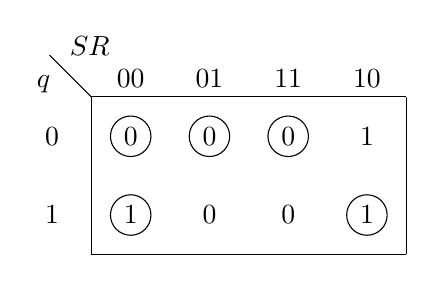
\begin{tikzpicture}
\pgfmathsetmacro{\kxstep}{1}
\pgfmathsetmacro{\kystep}{1}
\pgfmathsetmacro{\kpin}{0.75}
\foreach \x in {0,4}{\draw(\x*\kxstep,0)--++(0,-2*\kystep);}
\foreach \x in {0,2}{\draw(0,-\x*\kystep)--++(4*\kxstep,0);}
\draw(0,0)--++(135:\kpin)node[pos=0.75,above right]{$SR$}node[pos=0.75,below left]{$q$};
\foreach \kx/\ka in {0/00,1/01,2/11,3/10}{\draw(\kx*\kxstep+\kxstep/2,0)node[above]{$\ka$};}
\foreach \kx/\ka in {-1/0,0/{0},1/{0},2/{0},3/1}{\draw(\kx*\kxstep+\kxstep/2,-0.5*\kystep)node[]{$\ka$};}
\foreach \kx/\ka in {-1/1,0/{1},1/0,2/0,3/{1}}{\draw(\kx*\kxstep+\kxstep/2,-1.5*\kystep)node[]{$\ka$};}
\foreach \kx in {0,1,2}{\draw(\kx*\kxstep+0.5*\kxstep,-0.5*\kystep)node[draw,circle,inner sep=1pt]{$\phantom{00}$};}
\foreach \kx in {0,3}{\draw(\kx*\kxstep+0.5*\kxstep,-1.5*\kystep)node[draw,circle,inner sep=1pt]{$\phantom{00}$};}
\end{tikzpicture}
\caption{}
\end{subfigure}
\caption{ایس آر پلٹ }
\label{شکل_غیر_معاصر_ایس_آر_پلٹ_کا_عبوری}
\end{figure}
 حال کے متغیر \عددی{Q} کو بطور باز رسی اشارہ \عددی{q} استعمال کیا گیا ہے۔یوں حال کا متغیر \عددی{Q}، اندرونی مداخل \عددی{q} جبکہ بیرونی مداخل \عددی{S} اور \عددی{R} ہیں۔انہیں استعمال کرتے ہوئے (درج بالا مساوات کی مدد سے )  شکل-ج میں پیش  عبوری جدول حاصل کی گئی  جہاں جدول کے اندر \عددی{Q} کی قیمت درج ہے۔آئیے اس پلٹ کا تجزیہ اس کے عبوری جدول کی مدد سے کریں۔پلٹ کا جدول صداقت مندرجہ ذیل ہے۔
 

 %
 \begin{align*}
 \begin{array}{cc|cc}
 \toprule
 S&R&Q_{n+1}&\overline{Q}_{n+1}\\
 \midrule
 0&0&Q_n&\overline{Q}_n\\
 0&1&0&1\\
 1&0&1&0\\
 1&1&0&0\\
 \bottomrule
 \end{array}
\end{align*}
 جدول سے ظاہر ہے کہ جمع متمم گیٹ پر مبنی ایس آر پلٹ استعمال کرتے ہوئے دونوں مداخل بیکوقت بلند کرنے کی اجازت نہیں۔ دونوں مداخل بیکوقت بلند کرنے سے پلٹ کے مخارج \عددی{Q} اور \عددی{\overline{Q}} بیکوقت پست ہوں گے جبکہ ہر صورت ان کا آپس میں متضاد رہنا ضروری ہے۔درج ذیل مساوات پر پورا اترنے سے یہ شرط پوری ہو گی۔
 \begin{align}
 S\cdot R=0
 \end{align}
%
\begin{figure}
\centering
\begin{subfigure}{0.45\textwidth}
\centering
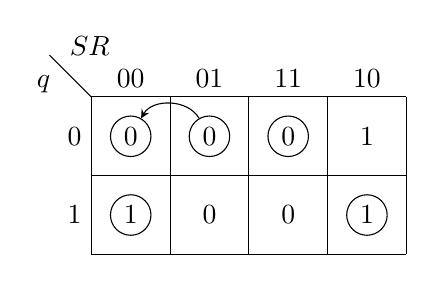
\begin{tikzpicture}
\pgfmathsetmacro{\kxstep}{1}
\pgfmathsetmacro{\kystep}{1}
\pgfmathsetmacro{\kpin}{0.75}
\def\ka{a}
\def\kb{b}
\pgfmathsetmacro{\ksepX}{2*\kxstep+2}
\foreach \x in {0,1,2,3,4}{\draw(\x*\kxstep,0)--++(0,-2*\kystep);}
\foreach \x in {0,1,2}{\draw(0,-\x*\kystep)--++(4*\kxstep,0);}
\draw(0,0)--++(135:\kpin)node[pos=0.75,above right]{$SR$}node[pos=0.75,below left]{$q$};
\foreach \kx/\xlb in {0/{00},1/{01},2/11,3/10}{\draw(\kx*\kxstep+\kxstep/2,0)node[above]{$\xlb$};}
\foreach \ky/\ylb in {0/0,1/1}{\draw(0,-\ky*\kystep-\kystep/2)node[left]{$\ylb$};}
\foreach \kx/\xlb in {0/0,1/0,2/0,3/1}{\draw(\kx*\kxstep+\kxstep/2,-\kystep/2)node[]{$\xlb$};}
\foreach \kx/\xlb in {0/1,1/0,2/0,3/1}{\draw(\kx*\kxstep+\kxstep/2,-1.5*\kystep)node[]{$\xlb$};}
\foreach \kx in {0,1,2}{\draw(\kx*\kxstep+\kxstep/2,-0.5*\kystep)node[draw,circle,inner sep=1pt](a\kx){$\phantom{00}$};}
\foreach \kx in {0,3}{\draw(\kx*\kxstep+\kxstep/2,-1.5*\kystep)node[draw,circle,inner sep=1pt](b\kx){$\phantom{00}$};}
\draw[-stealth](a1) to [out=120,in=60](a0);
\end{tikzpicture}
\caption{}
\end{subfigure}\hfill
\begin{subfigure}{0.45\textwidth}
\centering
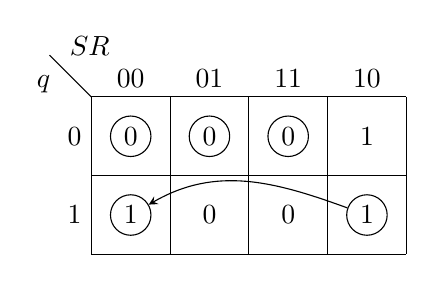
\begin{tikzpicture}
\pgfmathsetmacro{\kxstep}{1}
\pgfmathsetmacro{\kystep}{1}
\pgfmathsetmacro{\kpin}{0.75}
\def\ka{a}
\def\kb{b}
\pgfmathsetmacro{\ksepX}{2*\kxstep+2}
\foreach \x in {0,1,2,3,4}{\draw(\x*\kxstep,0)--++(0,-2*\kystep);}
\foreach \x in {0,1,2}{\draw(0,-\x*\kystep)--++(4*\kxstep,0);}
\draw(0,0)--++(135:\kpin)node[pos=0.75,above right]{$SR$}node[pos=0.75,below left]{$q$};
\foreach \kx/\xlb in {0/{00},1/{01},2/11,3/10}{\draw(\kx*\kxstep+\kxstep/2,0)node[above]{$\xlb$};}
\foreach \ky/\ylb in {0/0,1/1}{\draw(0,-\ky*\kystep-\kystep/2)node[left]{$\ylb$};}
\foreach \kx/\xlb in {0/0,1/0,2/0,3/1}{\draw(\kx*\kxstep+\kxstep/2,-\kystep/2)node[]{$\xlb$};}
\foreach \kx/\xlb in {0/1,1/0,2/0,3/1}{\draw(\kx*\kxstep+\kxstep/2,-1.5*\kystep)node[]{$\xlb$};}
\foreach \kx in {0,1,2}{\draw(\kx*\kxstep+\kxstep/2,-0.5*\kystep)node[draw,circle,inner sep=1pt](a\kx){$\phantom{00}$};}
\foreach \kx in {0,3}{\draw(\kx*\kxstep+\kxstep/2,-1.5*\kystep)node[draw,circle,inner sep=1pt](b\kx){$\phantom{00}$};}
\draw[-stealth](b3) to [out=160,in=30](b0);
\end{tikzpicture}
\caption{}
\end{subfigure}
\caption{ایس آر پلٹ کا استعمال}
\label{شکل_غیر_معاصر_ایس_آر_استعمال}
\end{figure} 

شکل  \حوالہ{شکل_غیر_معاصر_ایس_آر_استعمال}  پر نظر رکھ کر آگے پڑھیں۔عبوری جدول کی \عددی{SR=01} قطار اور \عددی{q=0} صف میں مستحکم حال پایا جاتا ہے جہاں حال کا متغیر پست \عددی{(Q=0)} ہے۔ عبوری جدول کے تحت \عددی{SR=00} کرنے سے حال کا متغیر پست رہے گا۔شکل -الف میں تیر دار لکیر اس عمل کو ظاہر کرتی ہے۔

اسی طرح \عددی{SR=10} کی صورت میں پلٹ کا  بلند مستحکم حال \عددی{q=1} کی صف میں پایا جاتا ہے۔عبوری جدول کے مطابق \عددی{SR=00} کرنے سے پلٹ بلند حال میں رہے گا  ، جو شکل-ب   میں تیر دار لکیر سے دکھایا گیا ہے۔یہ دونوں اعمال پلٹ کے بوولین جدول سے بھی واضح ہیں۔

اب دیکھتے ہیں \عددی{SR=11} سے آغاز کرتے ہوئے \عددی{SR=00} کرنے سے کیا صورت پیدا ہوتی ہے۔یاد رہے ان ادوار کو \موٹا{ بنیادی طریق کار }کے تحت چلایا جاتا ہے جہاں ایک سے زیادہ بیرونی مداخل تبدیل کرنے کی اجازت نہیں۔بہرحال پھر بھی دیکھتے ہیں کہ ایسا کرنے سے کیا مسائل کھڑے ہوتے ہیں۔بوولین جدول کے مطابق \عددی{SR=00}کرنے سے قبل \عددی{Q} اور \عددی{\overline{Q}} دونوں پست ہوں گے نا کہ آپس میں متضاد جبکہ کسی بھی پلٹ کے لئے لازم ہے کہ اس کے دونوں مخارج ہر وقت متضاد حال ہوں۔ساتھ ہی، عبوری جدول کے تحت اگر \عددی{S}پہلے پست حال اختیار کر لے تو اختتامی حال \عددی{0} ہو گا جبکہ اگر \عددی{R} پہلے پست ہو تب اختتامی حال \عددی{1} ہو گا۔چونکہ قبل از وقت یہ جاننا ممکن نہیں کہ \عددی{S} یا \عددی{R} پہلے پست ہو گا لہٰذا اختتامی حال جاننا ممکن نہیں۔ دور کا یوں استعمال غیر یقینی صورت پیدا کرے گا۔


\جزوحصہ{ ساعت کے کنارہ پر چلتا ہوا ڈی پلٹ}
شکل \حوالہ{شکل_غیر_معاصر_ڈی_پلٹ_بطور_باز_رسی}  -ا میں   ڈی پلٹ دکھایا گیا ہے جو ساعت کے کنارہ پر چلتا ہے۔ڈی پلٹ میں اندرونی باز رسی دور پایا جاتا ہے جس کے اندرونی حال کے متغیرات \عددی{S} اور \عددی{R} جبکہ باز رسی اشارات \عددی{s} اور \عددی{r} ہیں\حاشیہد{اس کتاب میں ضرب متمم گیٹ پر مبنی ایس آر پلٹ کے مداخل عموماً \عددی{\overline{S}} اور \عددی{\overline{R}} لکھے گئے ہیں۔ یہاں \عددی{S} اور \عددی{R} لکھا گیا ہے۔ امید کی جاتی ہے کہ اس سے پریشانی پیدا نہیں ہو گی۔}۔شکل -ب میں ڈی پلٹ کو باز رسی دور کے طرز پر بنایا گیا ہے تا کہ باز رسی اشارات \عددی{s} اور \عددی{r} کی پہچان آسان ہو۔

\begin{figure}
\centering
\begin{subfigure}{1\textwidth}
\centering
\begin{tikzpicture}
\pgfmathsetmacro{\kxstep}{1}
\pgfmathsetmacro{\kystep}{1}
\pgfmathsetmacro{\kpin}{0.5}
\pgfmathsetmacro{\ksepY}{2}
\draw(0,0) node[nand port,number inputs=2,anchor=out](u0){};
\draw(0,\ksepY) node[nand port,number inputs=2,anchor=out](u1){};
\draw(u0.out)--++(0,\kpin)coordinate(aa);
\draw(u1.out)--++(0,-\kpin)coordinate(bb);
\draw(u0.in 1)--++(0,\kpin)--(bb);
\draw(u1.in 2)--++(0,-\kpin)--(aa);
\draw (u0.out)--++(\kpin,0)node[right]{$\overline{Q}$};
\draw (u1.out)--++(\kpin,0)node[right]{$Q$};
\draw(u0.in 2)--++(-2*\kpin,0) node[nand port,number inputs=3,anchor=out](u3){};
\draw(u3.out)node[above right]{$R$}++(0,-\ksepY) node[nand port,number inputs=2,anchor=out](u4){};
\draw(u4.out)node[right]{$B$}--++(0,\kpin)coordinate(aa);
\draw(u3.out)--++(0,-\kpin)coordinate(bb);
\draw(u4.in 1)--++(0,\kpin)--(bb);
\draw(u3.in 3)--++(0,-\kpin)--(aa);
\draw(u1.in 1)--++(-2*\kpin,0) node[nand port,number inputs=2,anchor=out](u5){};
\draw(u5.out)node[above right]{$S$}node[draw,circle,minimum size=4pt,inner sep=0pt,fill=black]{}++(0,\ksepY) node[nand port,number inputs=2,anchor=out](u6){};
\draw(u5.out)--++(0,\kpin)coordinate(aa);
\draw(u6.out)node[right]{$A$}--++(0,-\kpin)coordinate(bb);
\draw(u5.in 1)--++(0,\kpin)--(bb);
\draw(u6.in 2)--++(0,-\kpin)--(aa);
\draw(u3.in 1)--++(0,\kpin)coordinate(cc);
\draw(u5.out)--++(0,-\kpin)--(cc);
\draw(u3.in 2)--++(-\kpin,0)|-(u5.in 2);
\draw($(u3.in 1)!0.5!(u5.in 2)$)++(-\kpin,0)--++(-2*\kpin,0)coordinate(kC)node[left]{$C$};
\draw(u4.in 2)--(u4.in 2 -| kC)node[left]{$D$};
\draw(u6.in 1)--++(-2*\kpin,0)coordinate(kT)--(kT |- u4.in 2)--++(0,-\kpin)-|(u4.out);
\draw(u1.out)node[shift={(-0.5cm,1cm)}]{\text{\RL{خارجی پلٹ}}};
\end{tikzpicture}
\caption{}
\end{subfigure}\hfill
\begin{subfigure}{1\textwidth}
\centering
\begin{tikzpicture}
\pgfmathsetmacro{\kxstep}{1}
\pgfmathsetmacro{\kystep}{1}
\pgfmathsetmacro{\kpin}{0.5}
\pgfmathsetmacro{\ksepY}{2}
\draw(0,0) node[nand port,number inputs=2,anchor=out](u0){};
\draw(0,\ksepY) node[nand port,number inputs=2,anchor=out](u1){};
\draw(u0.out)--++(0,\kpin)coordinate(aa);
\draw(u1.out)--++(0,-\kpin)coordinate(bb);
\draw(u0.in 1)--++(0,\kpin)--(bb);
\draw(u1.in 2)--++(0,-\kpin)--(aa);
\draw (u0.out)--++(\kpin,0)node[right]{$\overline{Q}$};
\draw (u1.out)--++(\kpin,0)node[right]{$Q$};
\draw(u0.in 2)--++(-4*\kpin,0)node[below right]{$R=\overline{BCs}$}node[nand port,number inputs=3,anchor=out](u2){};
\draw(u2.in 1)--++(0,\kpin)--++(-3*\kpin,0)node[above right]{$B=\overline{rD}$}node[nand port,number inputs=2,anchor=out](u3){};
\draw(u1.in 1)--++(-4*\kpin,0)node[above right]{$S=\overline{AC}$}node[nand port,number inputs=2,anchor=out](u4){};
\draw(u4.in 1)--++(0,\kpin)--++(-3*\kpin,0)node[above right]{$A=\overline{sB}$}node[nand port,number inputs=2,anchor=out](u5){};
\draw(u5.in 1)node[left]{$s$}--++(0,\kpin)-|(u4.out);
\draw(u3.in 1)node[left]{$r$}--++(0,\kpin)-|(u2.out);
\draw(u5.in 2)--++(-\kpin,0)coordinate(klft)node[left]{$B$};
\draw(u4.in 2)--(u4.in 2 -| klft)node[left]{$C$};
\draw(u3.in 2)--(u3.in 2 -| klft)node[left]{$D$};
\draw(u2.in 2)--(u2.in 2 -| klft)node[left]{$C$};
\draw(u2.in 3)--(u2.in 3 -| klft)node[left]{$s$};
\end{tikzpicture}
\caption{}
\end{subfigure}
\caption{ڈی پلٹ بطور باز رسی دور}
\label{شکل_غیر_معاصر_ڈی_پلٹ_بطور_باز_رسی}
\end{figure}

اس دور میں \عددی{S} اور \عددی{R} حال کے متغیرات ، \عددی{s} اور \عددی{r} باز رسی اشارات ، جبکہ \عددی{C} اور \عددی{D} بیرونی مداخل ہیں۔یوں درج ذیل لکھا جا سکتا ہے۔
\begin{gather}
\begin{aligned}
A&=\overline{sB}\\
B&=\overline{Dr}\\
S&=\overline{AC}=\overline{A}+\overline{C}=\overline{\overline{sB}}+\overline{C}=sB+\overline{C}=s(\overline{rD})+\overline{C}\\
&=s(\overline{r}+\overline{D})+\overline{C}\\
R&=\overline{BCs}=\overline{B}+\overline{C}+\overline{s}=\overline{\overline{Dr}}+\overline{C}+\overline{s}\\
&=Dr+\overline{C}+\overline{s}
\end{aligned}
\end{gather}

 ان مساوات سے حاصل \عددی{S} اور \عددی{R} کے بوولین جدول کو کارناف نقشہ جات کے  طرز پر شکل \حوالہ{شکل_غیر_معاصر_ڈی_پلٹ_عبوری_حصول}-ا  ا ور شکل-ب میں لکھ کر شکل   -ج  کا  عبوری جدول حاصل کیا گیا۔   \اصطلاح{مکمل حال }\فرہنگ{حال!مکمل}\حاشیہب{complete state}\فرہنگ{state!complete} \عددی{srCD} کی صورت میں لکھتے ہوئے اس جدول پر غور کرتے ہیں۔

\begin{figure}
\centering
\begin{subfigure}{0.45\textwidth}
\centering
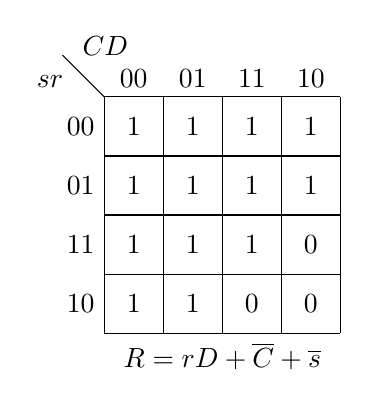
\begin{tikzpicture}
\pgfmathsetmacro{\kxstep}{0.75}
\pgfmathsetmacro{\kystep}{0.75}
\pgfmathsetmacro{\kpin}{0.75}
\pgfmathsetmacro{\ksepX}{2*\kxstep+2}
\foreach \x in {0,1,2,3,4}{\draw(\x*\kxstep,0)--++(0,-4*\kystep);}
\foreach \x in {0,1,2,3,4}{\draw(0,-\x*\kystep)--++(4*\kxstep,0);}
\draw(0,0)--++(135:\kpin)node[pos=0.75,above right]{$CD$}node[pos=0.75,below left]{$sr$};
\foreach \kx/\xlb in {0/{00},1/{01},2/11,3/10}{\draw(\kx*\kxstep+\kxstep/2,0)node[above]{$\xlb$};}
\foreach \ky/\ylb in {0/{00},1/{01},2/11,3/10}{\draw(0,-\ky*\kystep-\kystep/2)node[left]{$\ylb$};}
\foreach \kx/\xlb in {0/1,1/1,2/1,3/1}{\draw(\kx*\kxstep+\kxstep/2,-0.5*\kystep)node[]{$\xlb$};}
\foreach \kx/\xlb in {0/1,1/1,2/1,3/1}{\draw(\kx*\kxstep+\kxstep/2,-1.5*\kystep)node[]{$\xlb$};}
\foreach \kx/\xlb in {0/1,1/1,2/1,3/0}{\draw(\kx*\kxstep+\kxstep/2,-2.5*\kystep)node[]{$\xlb$};}
\foreach \kx/\xlb in {0/1,1/1,2/0,3/0}{\draw(\kx*\kxstep+\kxstep/2,-3.5*\kystep)node[]{$\xlb$};}
\draw(2*\kxstep,-4*\kystep)node[below]{$R=rD+\overline{C}+\overline{s}$};
\end{tikzpicture}
\caption{}
\end{subfigure}\hfill
\begin{subfigure}{0.45\textwidth}
\centering
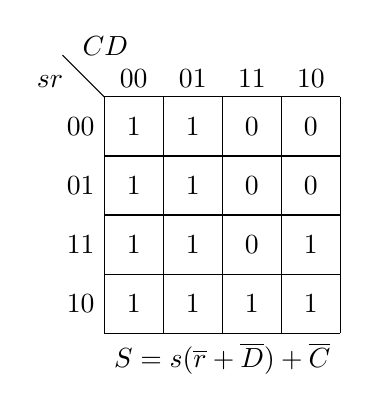
\begin{tikzpicture}
\pgfmathsetmacro{\kxstep}{0.75}
\pgfmathsetmacro{\kystep}{0.75}
\pgfmathsetmacro{\kpin}{0.75}
\pgfmathsetmacro{\ksepX}{2*\kxstep+2}
\foreach \x in {0,1,2,3,4}{\draw(\x*\kxstep,0)--++(0,-4*\kystep);}
\foreach \x in {0,1,2,3,4}{\draw(0,-\x*\kystep)--++(4*\kxstep,0);}
\draw(0,0)--++(135:\kpin)node[pos=0.75,above right]{$CD$}node[pos=0.75,below left]{$sr$};
\foreach \kx/\xlb in {0/{00},1/{01},2/11,3/10}{\draw(\kx*\kxstep+\kxstep/2,0)node[above]{$\xlb$};}
\foreach \ky/\ylb in {0/{00},1/{01},2/11,3/10}{\draw(0,-\ky*\kystep-\kystep/2)node[left]{$\ylb$};}
\foreach \kx/\xlb in {0/1,1/1,2/0,3/0}{\draw(\kx*\kxstep+\kxstep/2,-0.5*\kystep)node[]{$\xlb$};}
\foreach \kx/\xlb in {0/1,1/1,2/0,3/0}{\draw(\kx*\kxstep+\kxstep/2,-1.5*\kystep)node[]{$\xlb$};}
\foreach \kx/\xlb in {0/1,1/1,2/0,3/1}{\draw(\kx*\kxstep+\kxstep/2,-2.5*\kystep)node[]{$\xlb$};}
\foreach \kx/\xlb in {0/1,1/1,2/1,3/1}{\draw(\kx*\kxstep+\kxstep/2,-3.5*\kystep)node[]{$\xlb$};}
\draw(2*\kxstep,-4*\kystep)node[below]{$S=s(\overline{r}+\overline{D})+\overline{C}$};
\end{tikzpicture}
\caption{}
\end{subfigure}
\begin{subfigure}{1\textwidth}
\centering
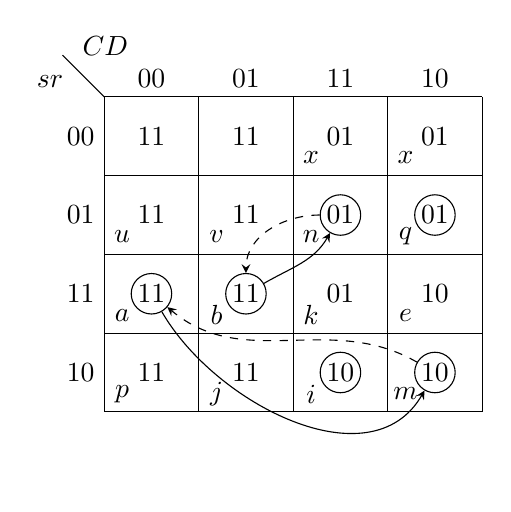
\begin{tikzpicture}
\pgfmathsetmacro{\kxstep}{1.2}
\pgfmathsetmacro{\kystep}{1}
\pgfmathsetmacro{\kpin}{0.75}
\pgfmathsetmacro{\ksepX}{2*\kxstep+2}
\foreach \x in {0,1,2,3,4}{\draw(\x*\kxstep,0)--++(0,-4*\kystep);}
\foreach \x in {0,1,2,3,4}{\draw(0,-\x*\kystep)--++(4*\kxstep,0);}
\draw(0,0)--++(135:\kpin)node[pos=0.75,above right]{$CD$}node[pos=0.75,below left]{$sr$};
\foreach \kx/\xlb in {0/{00},1/{01},2/11,3/10}{\draw(\kx*\kxstep+\kxstep/2,0)node[above]{$\xlb$};}
\foreach \ky/\ylb in {0/{00},1/{01},2/11,3/10}{\draw(0,-\ky*\kystep-\kystep/2)node[left]{$\ylb$};}
\foreach \kx/\xlb in {0/11,1/11,2/01,3/01}{\draw(\kx*\kxstep+\kxstep/2,-0.5*\kystep)node[]{$\xlb$};}
\foreach \kx/\xlb in {0/11,1/11,2/01,3/01}{\draw(\kx*\kxstep+\kxstep/2,-1.5*\kystep)node[]{$\xlb$};}
\foreach \kx/\xlb in {0/11,1/11,2/01,3/10}{\draw(\kx*\kxstep+\kxstep/2,-2.5*\kystep)node[]{$\xlb$};}
\foreach \kx/\xlb in {0/11,1/11,2/10,3/10}{\draw(\kx*\kxstep+\kxstep/2,-3.5*\kystep)node[]{$\xlb$};}
\foreach \kx/\xlb in {2,3}{\draw(\kx*\kxstep+\kxstep/2,-1.5*\kystep)node[draw,circle,inner sep=1pt](b\kx){$\phantom{00}$};}
\foreach \kx/\xlb in {0,1}{\draw(\kx*\kxstep+\kxstep/2,-2.5*\kystep)node[draw,circle,inner sep=1pt](c\kx){$\phantom{00}$};}
\foreach \kx/\xlb in {2,3}{\draw(\kx*\kxstep+\kxstep/2,-3.5*\kystep)node[draw,circle,inner sep=1pt](d\kx){$\phantom{00}$};}
\foreach \kx/\xlb in {0/{},1/{},2/x,3/x}{\draw(\kx*\kxstep,-1*\kystep)node[shift={(1.5ex,1.5ex)}]{$\xlb$};}
\foreach \kx/\xlb in {0/{u},1/{v},2/n,3/q}{\draw(\kx*\kxstep,-2*\kystep)node[shift={(1.5ex,1.5ex)}]{$\xlb$};}
\foreach \kx/\xlb in {0/{a},1/{b},2/k,3/e}{\draw(\kx*\kxstep,-3*\kystep)node[shift={(1.5ex,1.5ex)}]{$\xlb$};}
\foreach \kx/\xlb in {0/{p},1/{j},2/i,3/m}{\draw(\kx*\kxstep,-4*\kystep)node[shift={(1.5ex,1.5ex)}]{$\xlb$};}
\draw[-stealth,dashed](b2) to [out=180,in=90](c1);
\draw[-stealth](c1) to [out=30,in=-120](b2);
\draw[-stealth,dashed](d3) to [out=150,in=-40](c0);
\draw[-stealth](c0) to [out=-60,in=-120](d3);
\end{tikzpicture}
\caption{}
\end{subfigure}
\caption{ڈی پلٹ کے عبوری جدول کا حصول اور استعمال}
\label{شکل_غیر_معاصر_ڈی_پلٹ_عبوری_حصول}
\end{figure}


فرض کریں جس لمحے پلٹ کو برقی طاقت مہیا کر کے زندہ کیا جاتا ہے اس لمحے ساعت، \عددی{C}، اور بیرونی مداخل، \عددی{D} ،دونوں پست ہیں۔عبوری جدول کے مطابق دور \عددی{CD=00} کی قطار میں ہوگا۔اس قطار میں  پہلا خانہ  \عددی{0000}، دوسرا خانہ  \عددی{0100}، اور  چوتھا خانہ \عددی{1000} عبوری حال کے متغیر ظاہر کرتے ہیں۔ ان خانوں میں عبوری حال \عددی{SR=11} ہے۔تیسرا خانہ \عددی{1100}، مستحکم حال \عددی{SR=11} ظاہر کرتا ہے۔ اگر برقی طاقت کی فراہمی کے لمحے تاخیر ایسی ہوں کہ دور ان تین عبوری خانوں میں سے کسی ایک میں داخل ہو تو وہ یہاں سے جلد \عددی{sr=11} کی صف پہنچ کر مستحکم حال اختیار کر ے گا۔اگر زندہ ہوتے ہی دور سیدھا \عددی{1100} خانے میں داخل ہو تب وہ یہی رہے گا۔

اس کے برعکس برقی طاقت مہیا کرنے کے لمحے اگر \عددی{C=1} اور \عددی{D=1} ہو تب عبوری جدول کے مطابق دور \عددی{0111} یا \عددی{1011} مستحکم حال پہنچ کر یہی رہے گا، جبکہ \عددی{C=1} اور \عددی{D=0} کی صورت میں دور \عددی{0110} یا \عددی{1010} حال میں ہو گا۔

پست ساعت کی صورت میں حال کے متغیر \عددی{SR} کی قیمت \عددی{11} رہتی ہے۔عبوری جدول میں \عددی{CD=00} اور \عددی{CD=01} کی دو قطاریں اس حقیقت کو ظاہر کرتی ہیں جہاں تمام \عددی{SR} کی قیمت \عددی{11} ہے۔ہم جانتے ہیں ایس آر پلٹ کے دونوں مداخل بلند ہونے کی صورت میں پلٹ اپنا حال برقرار رکھتی ہے۔یوں شکل  \حوالہ{شکل_غیر_معاصر_ڈی_پلٹ_بطور_باز_رسی} میں خارجی پلٹ اپنا حال برقرار رکھے گی۔

پست ساعت، \عددی{C=0}، اور پست \عددی{D} کی صورت میں مستحکم حال کا متغیر \عددی{SR} حاصل کرنے کی خاطر ہم عبوری جدول کی \عددی{CD=00} قطار میں دیکھتے ہیں جہاں ہمیں \موٹا{ مکمل حال } \عددی{srCD=1100} بطور مستحکم حال ملتا ہے۔جدول کے اس خانے میں \عددی{a} لکھ کر اسے اجاگر کیا گیا ہے۔یہاں \عددی{SR=11} کی بدولت خارجی پلٹ اپنا حال برقرار رکھے گی۔

پست ساعت اور بلند \عددی{D} کی صورت میں \عددی{CD=01} کی قطار میں مستحکم حال \عددی{1101} پایا جاتا ہے جہاں \عددی{SR=11} ہے اور یوں خارجی پلٹ اپنا حال برقرار رکھے گی۔جدول کے اس خانے میں \عددی{b} لکھ کر اسے اجاگر کیا گیا ہے۔

فرض کریں دور مستحکم حال \عددی{1100}،یعنی خانہ \عددی{a} ،میں ہے جب بیرونی مداخل \عددی{C} بلند ہوتا ہے۔بیرونی مداخل \عددی{C} جس لمحہ \عددی{0} سے \عددی{1} ہوتا ہے اس لمحے کو ساعت کا \اصطلاح{کنارہ چڑھائی }\فرہنگ{کنارہ!چڑھائی}\حاشیہب{rising edge}\فرہنگ{edge!rising} کہتے ہیں۔ یوں \عددی{D=0} کی صورت میں ساعت کے کنارہ چڑھائی پر دور خانہ \عددی{a} کی صف میں رہتے ہوئے، \عددی{CD=00} سے \عددی{CD=10} کی قطار میں داخل ہو کر عبوری حال \عددی{1110} اختیار کرتا ہے۔اس عبوری حال کو خانہ \عددی{e} کہا گیا ہے، جہاں سے دور جلد اختتامی مستحکم حال \عددی{1010} پہنچے گا جس کو خانہ \عددی{m} ظاہر کرتا ہے۔ حال \عددی{1010} میں حال کا متغیر \عددی{SR=10} ہے۔خارجی پلٹ \عددی{SR=10} کی صورت میں پست حال اختیار کر ے گی لہٰذا \عددی{Q=0} ہو جائے گا۔اس قدم کو خانہ \عددی{a}سے خانہ \عددی{e} کے راستے خانہ \عددی{m} تک تیر دار لکیر سے ظاہر کیا گیا ہے۔ خلاصہ یہ ہے کہ \عددی{D=0} کی صورت میں ساعت کے کنارہ چڑھائی پر \عددی{Q=0} ہو جائے گا یعنی ڈی پلٹ پست حال اختیار کرے گی۔

اس پورے عمل پر دوبارہ غور کرتے ہیں۔ساعت کے کنارہ چڑھائی آتے ہی دور عبوری حال \عددی{1110} سے گزر کر مستحکم حال \عددی{1010} اختیار کرتا ہے۔ان دونوں حال میں \عددی{SR=10} رہتا ہے اور یوں عبوری حال سے گزرتے ہوئے لرزش پیدا نہیں ہوگی۔آگے پڑھتے ہوئے تسلی کر لیں کہ ہر قدم پر کسی بھی عبوری حال سے گزرتے وقت \عددی{SR} کی قیمت وہی ہو گی جو اس قدم کے اختتامی حال میں ہو گی۔یوں ان لمحات پر لرزش سے کسی قسم کی غیر یقینی صورت پیدا نہیں ہو گی۔

اسی طرح مکمل حال \عددی{srCD=1101} میں موجود دور ، ساعت کے کنارہ چڑھائی پر ، عبوری حال \عددی{1111} سے گزر کر مستحکم حال \عددی{0111} اختیار کرے گا۔اس قدم کو خانہ \عددی{b} سے خانہ \عددی{k} کے راستے خانہ \عددی{n} تک تیر دار لکیر ظاہر کرتی ہے۔یہ قدم بلند بیرونی مداخل \عددی{D=1} اور ساعت کے کنارہ چڑھائی پر \عددی{SR=01} کی صورت میں ہونے والا عمل ہے جس سے داخلی پلٹ بلند ہو کر ڈی پلٹ کا مخارج بلند \عددی{(Q=1)} کرتا ہے۔

ساعت کے \اصطلاح{ کنارہ اترائی } پر ہونے والے عمل کو  تیر دار لکیروں سے ظاہر کیا گیا ہے۔انہیں آپ خود سمجھ سکتے ہیں۔یہ دونوں لکیریں یہ حقیقت واضح کرتی ہیں کہ ساعت کے کنارہ اترائی پر عبوری حال اور اختتامی مستحکم حال دونوں میں \عددی{SR=11} ہو گا لہٰذا بیرونی پلٹ اپنا حال برقرار رکھے گی اور یوں ساعت کے کنارہ اترائی پر ڈی پلٹ کے حال میں کسی قسم کی تبدیلی رو نما نہیں ہوگی۔

ایک آخری بات اس پلٹ کے حوالے سے کرتے ہیں۔شکل  \حوالہ{شکل_غیر_معاصر_ڈی_پلٹ_بطور_باز_رسی}  میں \عددی{R} پیدا کرنے والے ضرب متمم گیٹ کو \عددی{S} بطور داخلی اشارہ مہیا کیا گیا ہے، جس کی بدولت \عددی{S} اور \عددی{R} کسی صورت بیکوقت پست نہیں ہو سکتے۔یاد رہے کہ \عددی{S} اور \عددی{R} دونوں بیکوقت پست ہونے سے بیرونی پلٹ کے دونوں مخارج بلند ہو جائیں گے جو کہ ناقابل قبول صورت ہو گی۔یوں عبوری جدول میں \عددی{0010} اور \عددی{0011} کے خانے کوئی معنی نہیں رکھتے۔ان خانوں کو \عددی{x} لکھ کر اجاگر کیا گیا ہے۔

\جزوحصہ{ایس آر پلٹوں پر مبنی غیر معاصر ادوار کا قدم با قدم تجزیہ}\شناخت{حصہ_غیر_معاصر_قدم_با_قدم}
مذکورہ بالا مثالوں میں استعمال کیے گئے طریقہ کار کو یہاں بیان کرتے ہیں۔پلٹ کے اپنے باز رسی اشارات کو نظر انداز کرتے ہیں۔
\begin{itemize}
\item
 تمام پلٹوں کے مخارج کو \عددی{Y_i}سے ظاہر کریں جہاں \عددی{i=0,1,2,\cdots}ہے۔ مخارج سے حاصل باز رسی اشارے کو اس مخارج کا \عددی{i} استعمال کرتے ہوئے \عددی{y_i} لکھیں۔ یوں \عددی{Y_3} سے حاصل باز رسی اشارہ \عددی{y_3} کہلائے گا۔
\item
 تمام پلٹوں کے \عددی{S_i} اور \عددی{R_i} مداخل کی مساوات حاصل کریں۔
\item
 جمع متمم گیٹ پر مبنی ایس آر پلٹ کے لئے تسلی کر لیں کہ \عددی{SR=0} ہے جبکہ ضرب متمم گیٹ پر مبنی ایس آر پلٹ کے لئے \عددی{\overline{S}\,\overline{R}=0} ہونا ضروری ہے۔ایسا نہ ہونے کی صورت میں پلٹ غلط نتائج دے سکتا ہے۔
\item 
\عددی{S_i} اور \عددی{R_i} دیکھ کر تمام پلٹ کے \عددی{Y_i} حاصل کریں۔
\item
 ہر \عددی{Y_i} کو کارناف نقشے کے طرز پر لکھیں۔ان نقشوں کی بائیں جانب قطار میں باز رسی اشارات \عددی{y} جبکہ نقشوں کے اُوپر صف میں بیرونی مداخل \عددی{x} لکھیں جہاں \عددی{y} سے مراد \عددی{\cdots y_3y_2y_1y_0} جبکہ \عددی{x} سے مراد \عددی{\cdots x_3x_2x_1x_0} ہے۔
\item
 ان نقشوں کو عبوری جدول میں یکجا کریں۔ ان نقشوں کے خانوں میں \عددی{Y} لکھیں، جہاں \عددی{Y} سے مراد \عددی{\cdots Y_3Y_2Y_1Y_0} ہے۔
\item
 وہ خانے جن میں \عددی{Y=y} ہو، مستحکم حال ظاہر کرتے ہیں۔انہیں دائرہ میں بند کریں۔یوں عبوری جدول حاصل ہو گا۔
\end{itemize}

